\documentclass{article}
\usepackage{amsmath}
\usepackage{graphicx}
\usepackage{listings}
\usepackage{xcolor}
\usepackage{float}

\lstset{
  language=Matlab,
  basicstyle=\ttfamily\small,
  keywordstyle=\color{blue},
  commentstyle=\color{green!50!black},
  numbers=left,
  numberstyle=\tiny,
  stepnumber=1,
  showstringspaces=false,
  frame=single,
  breaklines=true
}


\begin{document}

\begin{center}
\Large \textbf{Week 1 Report} \\
\large Ahmad Al Kadi
\end{center}
\vspace{0.25em}\hrule\vspace{1.0em}



\section{Introduction}

The purpose of this project is to apply fundamental concepts of
electromagnetic induction and AC circuit analysis to the study of a small AC
generator. The assignment is divided into three main exercises, each focusing
on a different stage of the process: from theoretical modeling, to analysis of
circuit elements, and finally the design of a complete measurement system.

\vspace{0.5cm}

In \textbf{Exercise 1}, the rotating coil generator is studied using
Faraday’s law. The magnetic flux and induced EMF are derived as functions of
time, the sinusoidal waveform properties are analyzed, and both analytical and
simulation results are compared.

\vspace{0.5cm}


\textbf{Exercise 2} extends the analysis to the three basic AC elements: the
resistor, inductor, and capacitor. For each case, the current response is
derived, instantaneous power is calculated, and the energy flow is discussed in
terms of dissipation or storage. Circuit diagrams and visualizations support
the interpretation.

\vspace{0.5cm}

Finally, in \textbf{Exercise 3}, a full measurement system is designed for the
generator operating under variable speed. The theoretical output is calculated,
appropriate instruments are selected, and a repeatable protocol is proposed.
Data acquisition and visualization are implemented with modern digital tools,
and an animated infographic is created to summarize the procedure.


\vspace{0.5cm}

Together, these three exercises form a complete workflow that links theory,
simulation, and experimental design. The report consolidates the results into a
structured format that demonstrates both the physical understanding of the
generator and the practical methods required for its measurement.





\section*{Exercise 1: Electromagnetic Induction and Faraday's Law}

\subsection*{Introduction}
A rectangular coil rotates in a uniform magnetic field. 
At $t=0$, the coil plane is perpendicular to the field (maximum flux). 
Given the data for Variant C:

\begin{itemize}
  \item Number of turns: $N = 100$
  \item Dimensions: $a = 0.06$ m, $b = 0.10$ m $\Rightarrow S = 0.006 \,\text{m}^2$
  \item Magnetic field: $B = 0.4$ T
  \item Rotation speed: $3000$ rpm $\Rightarrow \omega = 314.159 \,\text{rad/s}$
\end{itemize}

\section{Magnetic Flux as a Function of Time} % 1.1

General Formula:
\[
\varphi = B \cdot S_\alpha, \quad \text{with } S_\alpha = S \cos \alpha
\]

So, for a single loop:
\[
\varphi = B \cdot S \cos \alpha
\]

When the coil rotates with angular speed $\omega$, the angle is time-dependent:
\[
\alpha = \omega t \quad \Rightarrow \quad \varphi(t) = B \cdot S \cos(\omega t)
\]

For a coil of $N$ turns, the total flux linkage is:
\[
\Phi(t) = N \cdot \varphi(t) = N \, B \, S \cos(\omega t)
\]

\noindent
Substituting the Variant C values:
\[
N = 100, \quad S = 0.06 \times 0.10 = 0.006 \,\text{m}^2, \quad B = 0.4 \,\text{T}, \quad \omega = 314.159 \,\text{rad/s}
\]

\[
\boxed{\;\Phi(t) = 0.24 \cos(314.159\,t) \ \text{Wb}\;}
\]


\section{Induced EMF} % 2

From Faraday's law:
\[
e(t) = -\,N\,\frac{d\Phi}{dt}
\]

We already obtained the flux linkage:
\[
\Phi(t) = N\,B\,S\cos(\omega t)
\]
or, for the single-loop flux,
\[
\varphi(t)=B\,S\cos(\omega t),\qquad \Phi(t)=N\,\varphi(t).
\]

Differentiate the single-loop flux:
\[
\frac{d\varphi}{dt} = \frac{d}{dt}\big[B\,S\cos(\omega t)\big]
= -\,B\,S\,\omega\,\sin(\omega t).
\]

Multiply by $N$ (flux linkage) and apply Faraday's minus sign:
\[
e(t) = -\,N\,\frac{d\varphi}{dt}
= -\,N\big[-\,B\,S\,\omega\,\sin(\omega t)\big]
= N\,B\,S\,\omega\,\sin(\omega t).
\]

\noindent\textbf{Numerical form:}
\[
N=100,\quad B=0.4~\text{T},\quad S=0.006~\text{m}^2,\quad \omega=314.159~\text{rad/s}
\]
\[
E_{\max}=NBS\omega = 75.4~\text{V}\quad\Rightarrow\quad
\boxed{\,e(t)=75.4\,\sin(314.159\,t)\ \text{V}\, } 
\]


\section{Waveform Properties} % 3
From the induced EMF expression
\[
e(t) = NBS\omega \sin(\omega t),
\]
We can extract the key sinusoidal waveform properties:

\begin{itemize}
    \item \textbf{Peak value:}
    \[
    E_{\text{max}} = NBS\omega
    = 100 \times 0.4 \times (0.06 \times 0.10) \times 314.159
    \approx 75.4~\text{V}
    \]

    \item \textbf{RMS value:}
    \[
    E_{\text{rms}} = \frac{E_{\text{max}}}{\sqrt{2}}
    = \frac{75.4}{\sqrt{2}} \approx 53.3~\text{V}
    \]

    \item \textbf{Frequency:}
    \[
    f = \frac{\omega}{2\pi} = \frac{314.159}{2\pi} \approx 50~\text{Hz}
    \]

    \item \textbf{Period:}
    \[
    T = \frac{1}{f} = \frac{1}{50} = 0.02~\text{s}
    \]
\end{itemize}


\section{Visualizations of Flux and EMF} % 4

The time variation of the magnetic flux and induced EMF was obtained 
using MATLAB. Figure~\ref{fig:flux_emf} shows the waveforms over one 
period of the sinusoidal cycle.

\begin{figure}[H]
    \centering
    \includegraphics[width=0.9\textwidth]{flux_emf.png}
    \caption{Magnetic flux $\Phi(t)$ and induced EMF $e(t)$ versus time.}
    \label{fig:flux_emf}
\end{figure}





\subsection{Sample Values} % 1.4

The induced EMF values at specific times can be obtained by substituting 
the time instants into the expression
\[
e(t) = E_{\text{max}} \sin(\omega t), \quad
E_{\text{max}} = 75.4~\text{V}, \quad \omega = 314.159~\text{rad/s}.
\]

\begin{align*}
e(0.001) &= 75.4 \cdot \sin(314.159 \cdot 0.001) \approx 23.3~\text{V}, \\
e(0.004) &= 75.4 \cdot \sin(314.159 \cdot 0.004) \approx 71.7~\text{V}, \\
e(0.008) &= 75.4 \cdot \sin(314.159 \cdot 0.008) \approx 44.3~\text{V}.
\end{align*}

These computed values are summarized in Table~\ref{tab:sample_values}.

\begin{table}[h]
\centering
\begin{tabular}{|c|c|}
\hline
$t$ (s) & $e(t)$ (V) \\
\hline
0.001 & 23.3 \\
0.004 & 71.7 \\
0.008 & 44.3 \\
\hline
\end{tabular}
\caption{Induced EMF values at selected times.}
\label{tab:sample_values}
\end{table}




\subsection{Calculations (MATLAB)} % 1.4.2

The following MATLAB script was used to compute the flux and emf
waveforms:

\begin{lstlisting}[language=Matlab]
% Exercise 1 – Variant C
N   = 100;          % turns
a   = 0.06;         % m
b   = 0.10;         % m
B   = 0.4;          % tesla
rpm = 3000;         % rev/min

S     = a*b;                    
omega = 2*pi*rpm/60;             
Emax  = N*B*S*omega;

t = [0.001, 0.004, 0.008];
e = Emax*sin(omega*t);

disp([t' e'])   % display results
\end{lstlisting}

The MATLAB output gives the induced EMF values:
\[
e(0.001) \approx 23.3~\text{V}, \quad
e(0.004) \approx 71.7~\text{V}, \quad
e(0.008) \approx 44.3~\text{V}
\]


\section{Generator System (Simulink)}

\begin{figure}[H]
    \centering
    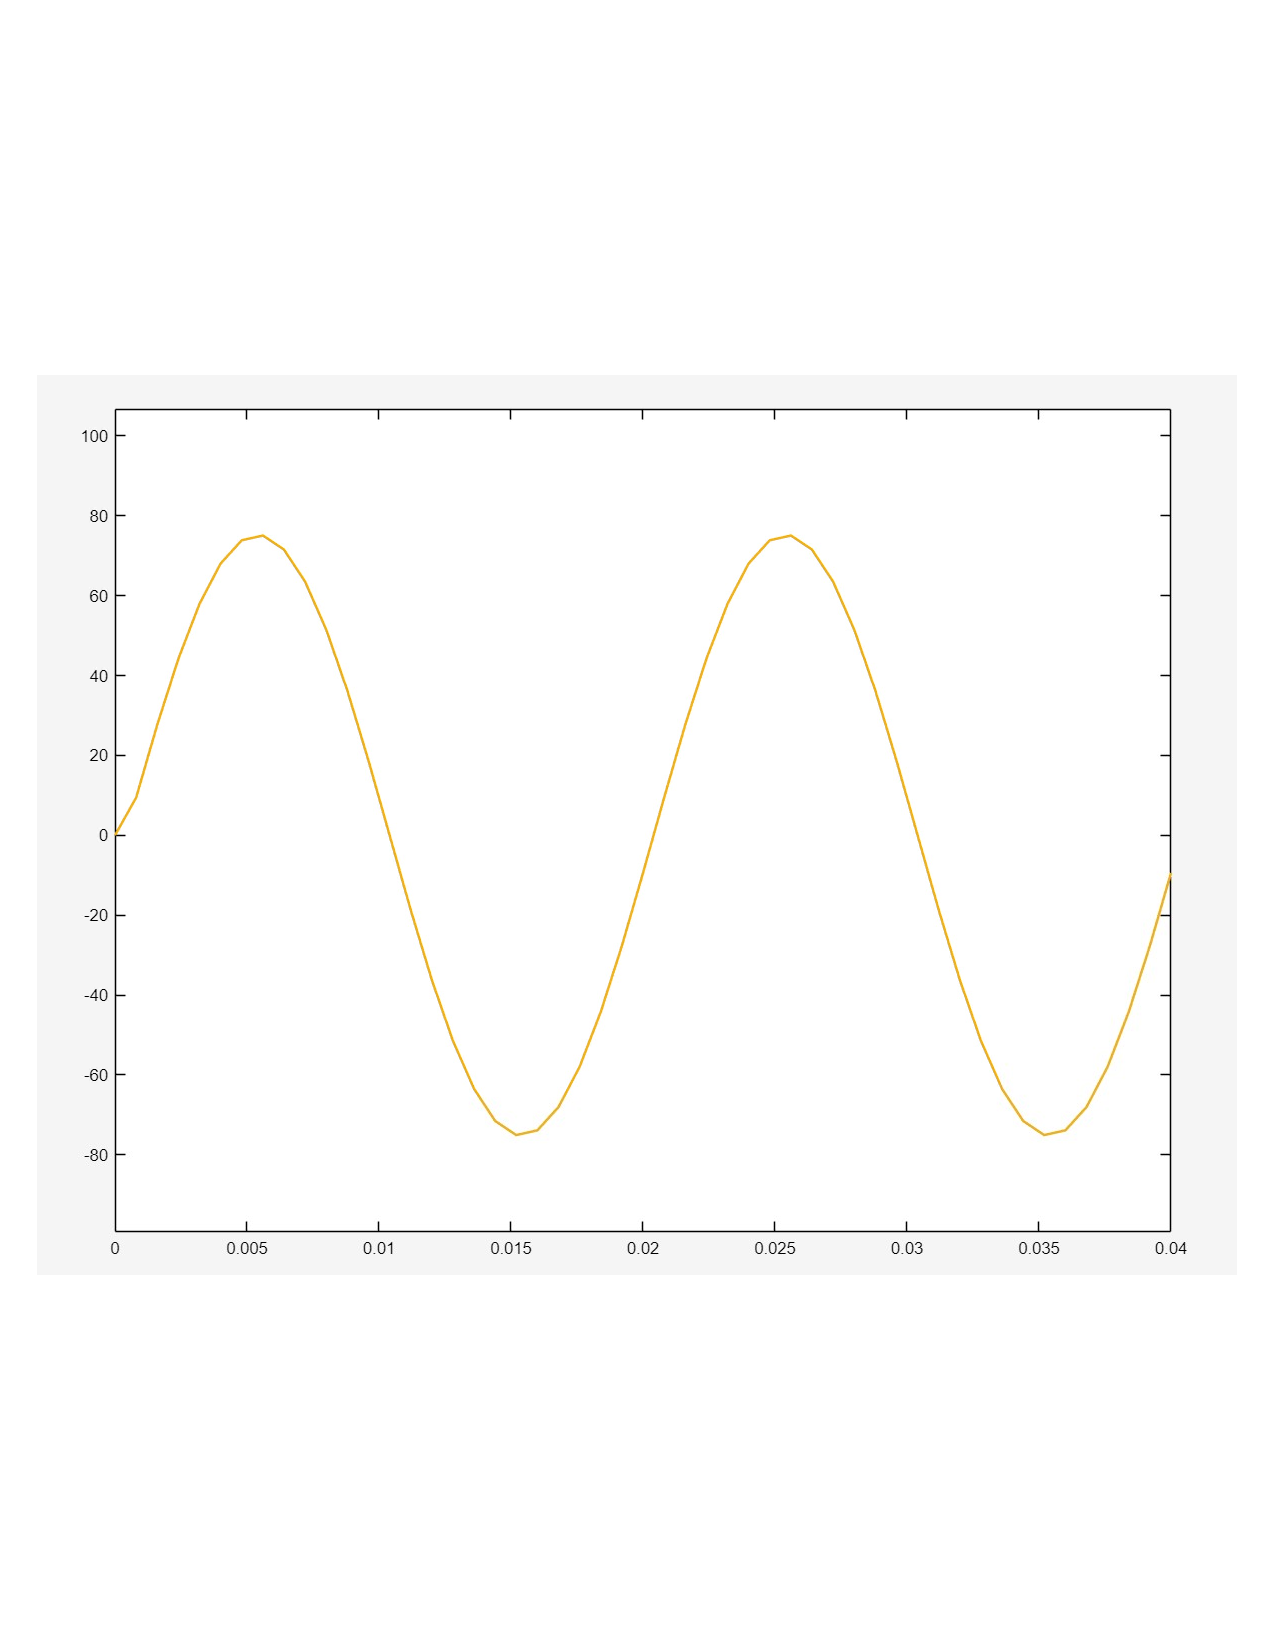
\includegraphics[width=0.9\textwidth]{Generator system.pdf}
    \caption{Simulink Scope output of the generator system showing the induced EMF $e(t)$ versus time.}
    \label{fig:simulink_emf}

\end{figure}
\noindent
The Simulink model was built using a Sine Wave (flux), Derivative, and Gain block to represent $e(t)=-N \frac{d\Phi}{dt}$. 
The Scope output shows the induced EMF as a sinusoidal waveform with peak amplitude $\approx 75$ V, matching the theoretical value.

 \vspace{+4cm}


\section{Interactive Plotly graph}
\begin{figure}[H]
    \centering
    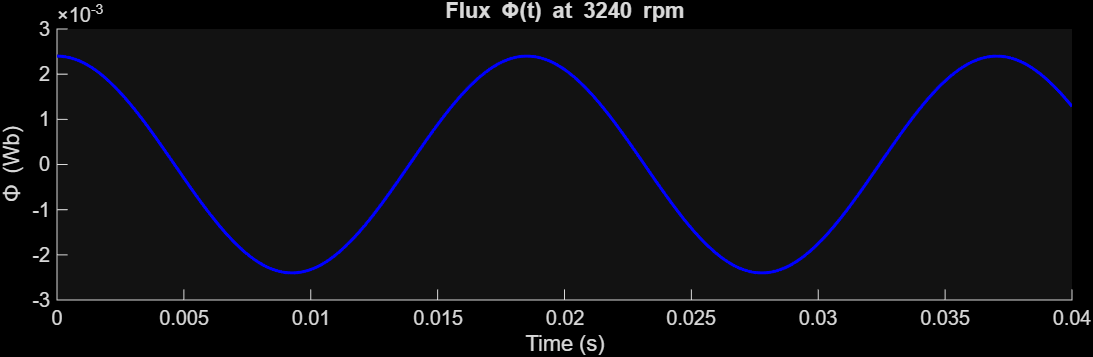
\includegraphics[width=0.9\textwidth]{flux_interactive.png}
    \caption{Interactive MATLAB app: Flux $\Phi(t)$ at 3240 rpm.}
    \label{fig:interactive_flux}
\end{figure}

\begin{figure}[H]
    \centering
    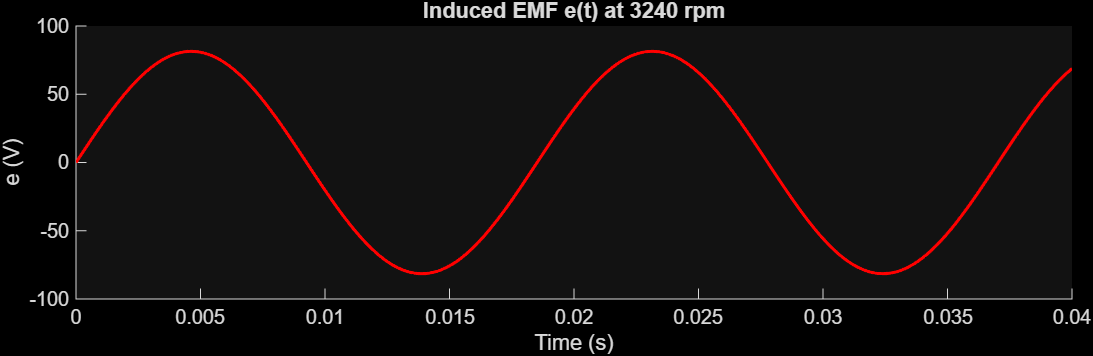
\includegraphics[width=0.9\textwidth]{emf_interactive.png}
    \caption{Interactive MATLAB app: Induced EMF $e(t)$ at 3240 rpm.}
    \label{fig:interactive_emf}
\end{figure}

\noindent
Additionally, an interactive MATLAB graph was developed to visualize the effect of rotation speed on the flux $\Phi(t)$ and induced EMF $e(t)$. 
The app consists of two real-time plots (flux and EMF) linked to a slider that adjusts the coil speed in rpm. 
By moving the slider, the user can directly observe how the frequency and amplitude of $e(t)$ vary according to 
$e(t) = -N \tfrac{d\Phi}{dt} = NBS\omega \sin(\omega t)$, thus confirming the theoretical dependence on angular velocity.









\newpage
\section*{Exercise 2: AC Circuit Elements Analysis}

\subsection*{Introduction}

In this exercise we analyze the behavior of the three fundamental AC elements — 
the resistor, the inductor, and the capacitor — when connected individually to 
a sinusoidal voltage source. 

The applied voltage is:

\[
v(t) = 80 \,\sin(628t)\ \text{V}
\]

with angular frequency $\omega = 628 \,\text{rad/s}$ corresponding to 
a frequency of $f = \tfrac{\omega}{2\pi} \approx 100 \,\text{Hz}$.

The objective of this problem is to:

\begin{itemize}
    \item Derive the current expressions $i(t)$ for each element using the 
    fundamental relations provided in the course notes (Ohm’s law for resistors, 
    the voltage–current law for inductors, and the voltage–current law for capacitors).
    \item Calculate the instantaneous power $p(t) = v(t)\,i(t)$ in each case.
    \item Analyze the nature of the energy flow, distinguishing between 
    dissipation (resistor) and storage (inductor, capacitor).
    \item Provide clear visualizations of voltage, current, and power for all 
    three elements.
\end{itemize}

This introduction establishes the framework for the following sections, where 
the analysis will be carried out step by step using only the formulas derived 
in the \textit{Mono.pdf} lecture notes.


\section*{2.1 \; Current expressions $i(t)$ for each element}

\noindent\textbf{Data:}
\[
v(t) = 80 \,\sin(628t)\ \text{V}, \quad \omega = 628 \,\text{rad/s}.
\]

From the assignment statement, we know:
\[
R = 40~\Omega, \qquad L = 0.1~\text{H}, \qquad C = 50~\mu\text{F}.
\]

Here $50~\mu\text{F}$ means “fifty microfarads.” Since the prefix $\mu$ means $10^{-6}$, we rewrite:
\[
C = 50 \times 10^{-6}\ \text{F} = 0.000050\ \text{F}.
\]

---

\subsection*{Element laws from the notes}

For each element, the course notes provide the fundamental time–domain equations:

\[
\text{Resistor: } u(t) = R \, i(t),
\]
\[
\text{Inductor: } u(t) = L \,\frac{di(t)}{dt},
\]
\[
\text{Capacitor: } i(t) = C \,\frac{du(t)}{dt}.
\]

Here $u(t)$ is the instantaneous voltage across the element, and $i(t)$ is the instantaneous current through it. In this exercise, $u(t)=v(t)=80\sin(628t)$ is the same for all three cases, because each element is connected directly to the given source.

---

\subsection*{(a) Resistor $R=40~\Omega$}

Start with $u(t) = R\,i_R(t)$.  
Solve for the current:
\[
i_R(t) = \frac{u(t)}{R}.
\]

Substitute the given data:  
\[
i_R(t) = \frac{80\sin(628t)}{40}.
\]

Simplify:
\[
i_R(t) = 2.00\,\sin(628t)\ \text{A}.
\]

\textbf{Result:} The resistor current has a peak value of $2.00$ A and is \emph{in phase} with the voltage.

---

\subsection*{(b) Inductor $L=0.1~\text{H}$}

Law: $u(t) = L \dfrac{di_L}{dt}$.  
Rearrange:
\[
\frac{di_L}{dt} = \frac{u(t)}{L}.
\]

Substitute the values: $u(t)=80\sin(628t)$ and $L=0.1$ H:
\[
\frac{di_L}{dt} = \frac{80\sin(628t)}{0.1} = 800\,\sin(628t).
\]

Now integrate to get $i_L(t)$:
\[
i_L(t) = \int 800\,\sin(628t)\,dt.
\]

The integral of $\sin(628t)$ is $-\frac{1}{628}\cos(628t)$, so:
\[
i_L(t) = -\frac{800}{628}\cos(628t) + K,
\]
where $K$ is a constant of integration.

In steady sinusoidal regime, there is no DC offset, so $K=0$.

Thus:
\[
i_L(t) = -1.274\,\cos(628t).
\]

Using the identity $-\cos(\theta)=\sin(\theta-\tfrac{\pi}{2})$, we write:
\[
i_L(t) = 1.274\,\sin\!\Big(628t - \frac{\pi}{2}\Big)\ \text{A}.
\]

\textbf{Result:} The inductor current has a peak of $1.274$ A and \emph{lags the voltage by $90^\circ$}, as expected.

---

\subsection*{(c) Capacitor $C=50~\mu\text{F}$}

Law: $i_C(t) = C \,\dfrac{du}{dt}$.

Differentiate $u(t) = 80\sin(628t)$:
\[
\frac{du}{dt} = 80 \cdot 628 \cos(628t) = 50240\,\cos(628t).
\]

Now multiply by $C$:
\[
i_C(t) = (50 \times 10^{-6}) \cdot 50240 \,\cos(628t).
\]

Calculate:
\[
i_C(t) = 2.512\,\cos(628t).
\]

Using $\cos(\theta)=\sin(\theta+\tfrac{\pi}{2})$:
\[
i_C(t) = 2.512\,\sin\!\Big(628t + \frac{\pi}{2}\Big)\ \text{A}.
\]

\textbf{Result:} The capacitor current has a peak of $2.512$ A and \emph{leads the voltage by $90^\circ$}, which matches the theoretical behavior of capacitors in AC.

---

\subsection*{Summary}

\[
\begin{array}{c|c|c}
\text{Element} & i(t) & \text{Phase relation w.r.t.\ } v(t) \\ \hline
R & 2.00\,\sin(628t)\ \text{A} & In phase ($0^\circ$) \\
L & 1.274\,\sin(628t-\tfrac{\pi}{2})\ \text{A} & Lags by $90^\circ$ \\
C & 2.512\,\sin(628t+\tfrac{\pi}{2})\ \text{A} & Leads by $90^\circ$ \\
\end{array}
\]

\vspace{0.5cm}

We can clearly see the three classical behaviors:
\vspace{0.5cm}

- Resistor: current aligns with voltage.
\\ 
- Inductor: current lags by one quarter of a cycle.
\\ 
- Capacitor: current leads by one quarter of a cycle.



\subsection*{Calculations (MATLAB) --- Section 2.1}

The following MATLAB script was used to compute the peak and RMS currents
for each element of Variant C. It also confirms the expected phase relation
between the voltage $v(t)$ and the current $i(t)$.

\begin{lstlisting}[language=Matlab]
% Exercise 2.1 — Variant C
% Source: v(t) = Vm*sin(omega*t)

Vm    = 80;      % volts (peak)
omega = 628;     % rad/s  (~100 Hz)

% Element values
R = 40;          % ohms
L = 0.1;         % henry
C = 50e-6;       % farad (50 microfarads)

% Reactances
XL = omega*L;
XC = 1/(omega*C);

% Peak currents
IR_peak = Vm/R;
IL_peak = Vm/XL;
IC_peak = Vm/XC;

% RMS currents
IR_rms = IR_peak/sqrt(2);
IL_rms = IL_peak/sqrt(2);
IC_rms = IC_peak/sqrt(2);

% Display results
fprintf('Resistor:  I_peak = %.3f A,  I_rms = %.3f A,  phase = 0 deg (in phase)\n', IR_peak, IR_rms);
fprintf('Inductor:  I_peak = %.3f A,  I_rms = %.3f A,  phase = -90 deg (lags)\n', IL_peak, IL_rms);
fprintf('Capacitor: I_peak = %.3f A,  I_rms = %.3f A,  phase = +90 deg (leads)\n', IC_peak, IC_rms);
\end{lstlisting}

The MATLAB output confirms the analytical results:
\[
\begin{aligned}
&\text{Resistor: } I_{\text{peak}} = 2.000~\text{A},\quad I_{\text{rms}} = 1.414~\text{A},\ \text{phase} = 0^\circ \ (\text{in phase}),\\[6pt]
&\text{Inductor: } I_{\text{peak}} = 1.274~\text{A},\quad I_{\text{rms}} = 0.901~\text{A},\ \text{phase} = -90^\circ \ (\text{lags}),\\[6pt]
&\text{Capacitor: } I_{\text{peak}} = 2.512~\text{A},\quad I_{\text{rms}} = 1.776~\text{A},\ \text{phase} = +90^\circ \ (\text{leads}).
\end{aligned}
\]

\noindent
These numerical values match the expressions obtained in the derivations of Section 2.1.

\vspace{0.5cm}

\section*{2.2 \; Instantaneous Power $p(t)$}

\noindent\textbf{Variant C:}
\[
v(t)=80\,\sin(628t)\ \text{V},\qquad \omega=628\ \text{rad/s}.
\]

\noindent\textbf{Definition used:} the instantaneous power on an element is
\[
\boxed{\,p(t)=v(t)\,i(t)\,}.
\]
For each element we multiply the same applied voltage $v(t)$ by the current $i(t)$
\emph{found previously in 2.1} from the element equations.

\vspace{0.8em}
\subsection*{(a) Resistor $R=40\,\Omega$}

\noindent\textbf{Current from 2.1:} 
\[
i_R(t)=\frac{v(t)}{R}=\frac{80}{40}\sin(628t)=2.00\,\sin(628t)\ \text{A}.
\]

\noindent\textbf{Power:} by definition,
\[
\begin{aligned}
p_R(t)&=v(t)\,i_R(t)=\big[80\sin(628t)\big]\big[2.00\sin(628t)\big]\\
      &=160\,\sin^2(628t)\ \text{W}.
\end{aligned}
\]

\noindent\textbf{Trig identity used:} 
\[
\sin^2\alpha=\frac{1}{2}\big(1-\cos 2\alpha\big).
\]
Apply it with $\alpha=628t$:
\[
\boxed{\,p_R(t)=80\,[\,1-\cos(1256t)\,]\ \text{W}.}
\]

\noindent\textbf{Results:}
\\
- The \(\cos(1256t)\) term has zero average over any full period, so the average power is
  \(\overline P_R=80\ \text{W}\).
  \\
- Instantaneous range: \(0\le p_R(t)\le 160\ \text{W}\). (Always non-negative → pure dissipation.)

\vspace{0.8em}
\subsection*{(b) Inductor $L=0.1\,\text{H}$}

\noindent\textbf{Current from 2.1 (obtained by integrating $u=L\,di/dt$):}
\[
i_L(t)=1.274\,\sin\!\Big(628t-\frac{\pi}{2}\Big)\ \text{A}.
\]
Here the numeric amplitude \(1.274\) comes from
\[
I_{Lm}=\frac{V_m}{\omega L}=\frac{80}{628\cdot 0.1}=\frac{80}{62.8}=1.274\ \text{A}.
\]

\noindent\textbf{Power:}
\[
p_L(t)=v(t)\,i_L(t)=80\sin(628t)\cdot 1.274\sin\!\Big(628t-\frac{\pi}{2}\Big).
\]

\noindent\textbf{Product identity used:}
\[
\sin A\,\sin B=\frac{1}{2}\big[\cos(A-B)-\cos(A+B)\big].
\]
Take \(A=628t\), \(B=628t-\tfrac{\pi}{2}\):
\[
\begin{aligned}
p_L(t)
&=\tfrac12(80)(1.274)\Big[\cos\!\Big(\tfrac{\pi}{2}\Big)-\cos\!\Big(1256t-\tfrac{\pi}{2}\Big)\Big]\\
&=\tfrac12(80)(1.274)\big[0-\sin(1256t)\big]\\
&=\boxed{\, -\,50.96\,\sin(1256t)\ \text{W}.}
\end{aligned}
\]
(The second line uses \(\cos(\tfrac{\pi}{2})=0\) and \(\cos(x-\tfrac{\pi}{2})=\sin x\).)

\noindent\textbf{Results:}
\\
- Amplitude \(= \dfrac{V_m I_{Lm}}{2}=\dfrac{80\cdot1.274}{2}=50.96\ \text{W}\).
\\
- Average power \(\overline P_L=0\) (ideal inductor stores/returns energy; signs alternate).

\vspace{0.8em}
\subsection*{(c) Capacitor $C=50\,\mu\text{F}=50\times10^{-6}\ \text{F}$}

\noindent\textbf{Where the value comes from:} \(50~\mu\text{F}\) means \(50\times 10^{-6}\) farads (prefix \(\mu=10^{-6}\)).

\noindent\textbf{Current from 2.1 (obtained by $i=C\,du/dt$):}
\[
i_C(t)=2.512\,\sin\!\Big(628t+\frac{\pi}{2}\Big)\ \text{A},
\]
with amplitude from
\[
I_{Cm}=\omega C V_m=(628)\,(50\times10^{-6})\,(80)=2.512\ \text{A}.
\]

\noindent\textbf{Power:}
\[
p_C(t)=v(t)\,i_C(t)=80\sin(628t)\cdot 2.512\sin\!\Big(628t+\frac{\pi}{2}\Big).
\]

\noindent\textbf{Use the same product identity} with \(A=628t\), \(B=628t+\tfrac{\pi}{2}\):
\[
\begin{aligned}
p_C(t)
&=\tfrac12(80)(2.512)\Big[\cos\!\Big(-\tfrac{\pi}{2}\Big)-\cos\!\Big(1256t+\tfrac{\pi}{2}\Big)\Big]\\
&=\tfrac12(80)(2.512)\big[0+\sin(1256t)\big]\\
&=\boxed{\, +\,100.48\,\sin(1256t)\ \text{W}.}
\end{aligned}
\]
(We used \(\cos(-\tfrac{\pi}{2})=0\) and \(\cos(x+\tfrac{\pi}{2})=-\sin x\).)

\noindent\textbf{Results:}
\\
- Amplitude \(= \dfrac{V_m I_{Cm}}{2}=\dfrac{80\cdot2.512}{2}=100.48\ \text{W}\).
\\
- Average power \(\overline P_C=0\) (ideal capacitor stores/returns energy).

\vspace{0.8em}
\subsection*{Summary}
\[
\begin{array}{c|c|c}
\text{Element} & p(t) & \text{Average over a period} \\\hline
R & 80\,[1-\cos(1256t)]\ \text{W} & 80~\text{W} \\
L & -\,50.96\,\sin(1256t)\ \text{W} & 0 \\
C & +\,100.48\,\sin(1256t)\ \text{W} & 0 \\
\end{array}
\]
All constants (80, 50.96, 100.48) come from multiplying the given voltage amplitude 
$V_m=80$ by the corresponding current amplitudes from 2.1 and the 
$\tfrac12$ factor in the trigonometric product identity.

\vspace{0.5cm}

\subsection*{Calculations (MATLAB) --- Section 2.2}

The following MATLAB script computes the instantaneous powers
\(
p_R(t)=v(t)i_R(t),\;
p_L(t)=v(t)i_L(t),\;
p_C(t)=v(t)i_C(t)
\)
for the values given and verifies the average powers over one period.

\begin{lstlisting}[language=Matlab]
% exercise2_2_power.m  -- Instantaneous power for R, L, C (Variant C)

Vm    = 80;            % V (peak)
omega = 628;           % rad/s
f     = omega/(2*pi);  % Hz
T     = 1/f;           % s

R = 40;        % ohm
L = 0.1;       % H
C = 50e-6;     % F

% Current amplitudes from Section 2.1
IR_peak = Vm/R;                 % 2.000 A (in phase)
IL_peak = Vm/(omega*L);         % 1.274 A (lags 90 deg)
IC_peak = Vm*(omega*C);         % 2.512 A (leads 90 deg)

phi_R = 0;      phi_L = -pi/2;  phi_C = +pi/2;

% Time base (two periods)
t = linspace(0, 2*T, 4000);

% v(t), i(t)
v  = Vm * sin(omega*t);
iR = IR_peak * sin(omega*t + phi_R);
iL = IL_peak * sin(omega*t + phi_L);
iC = IC_peak * sin(omega*t + phi_C);

% Instantaneous power
pR = v .* iR;   pL = v .* iL;   pC = v .* iC;

% Theoretical references
PR_avg_theory = (Vm^2)/(2*R);     % 80.00 W
PL_amp_theory = (Vm*IL_peak)/2;   % 50.96 W
PC_amp_theory = (Vm*IC_peak)/2;   % 100.48 W

% Numerical averages over one period
idx = t >= T & t <= 2*T;
PR_avg_num = mean(pR(idx));
PL_avg_num = mean(pL(idx));
PC_avg_num = mean(pC(idx));

% Display
fprintf('--- Instantaneous Power Results (Variant C) ---\n');
fprintf('Resistor:   p_R(t) = 80*(1 - cos(1256 t)) W\n');
fprintf('  Average power (theory)   = %.2f W\n', PR_avg_theory);
fprintf('  Average power (numeric)  = %.2f W\n\n', PR_avg_num);

fprintf('Inductor:   p_L(t) = -%.2f*sin(1256 t) W (avg = 0)\n', PL_amp_theory);
fprintf('  Average power (numeric)  = %.2f W\n\n', PL_avg_num);

fprintf('Capacitor:  p_C(t) = +%.2f*sin(1256 t) W (avg = 0)\n', PC_amp_theory);
fprintf('  Average power (numeric)  = %.2f W\n\n', PC_avg_num);
\end{lstlisting}

The script outputs the following values, which confirm the analytical results:
\[
\begin{aligned}
&\text{Resistor: } \overline P_R = 80.00~\text{W} \ \text{(theory)},\quad
\overline P_R \approx 79.98~\text{W} \ \text{(numeric)},\\[4pt]
&\text{Inductor: } p_L(t) = -50.96\,\sin(1256t)\ \text{W},\quad
\overline P_L \approx 0~\text{W},\\[4pt]
&\text{Capacitor: } p_C(t) = +100.48\,\sin(1256t)\ \text{W},\quad
\overline P_C \approx 0~\text{W}.
\end{aligned}
\]

\noindent
The waveforms of $v(t)$, $i(t)$ and $p(t)$ for the three elements are shown in
Figure~\ref{fig:power_RLC}, exported from MATLAB.

\begin{figure}[H]
    \centering
    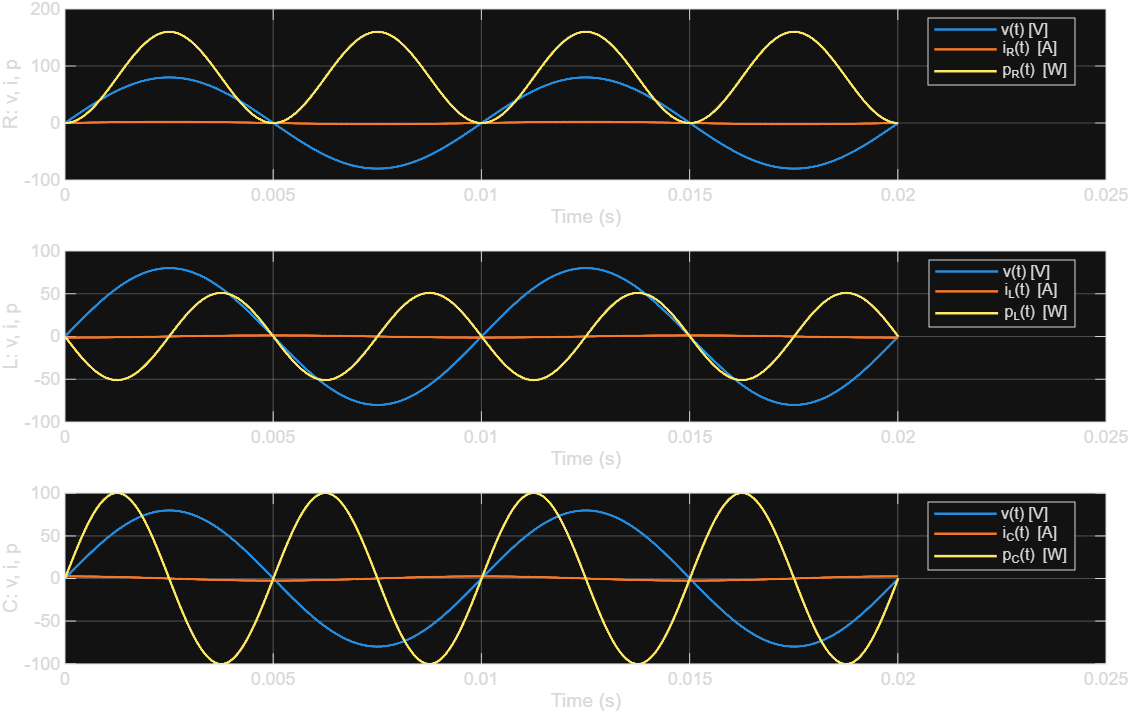
\includegraphics[width=0.9\textwidth]{Instantaneous Power.png}
    \caption{Instantaneous power waveforms for resistor, inductor, and capacitor (Variant C). 
             Each subplot shows the source voltage $v(t)$, element current $i(t)$, 
             and instantaneous power $p(t)=v(t)i(t)$.}
    \label{fig:power_RLC}
\end{figure}


\newpage
\section*{2.3 \; Analyze Energy Flow (consumption vs.\ storage)}

\noindent\textbf{Given:}
\[
v(t)=80\,\sin(628t)\ \text{V},\qquad \omega=628\ \text{rad/s},\qquad
R=40~\Omega,\; L=0.1~\text{H},\; C=50~\mu\text{F}=50\times10^{-6}\ \text{F}.
\]
(\(\mu\) means \(10^{-6}\).)

\noindent\textbf{Element laws already used in 2.1:}
\[
u=Ri,\quad u=L\,\frac{di}{dt},\quad i=C\,\frac{du}{dt}\ \ \,
\]
Instantaneous power is defined as \(p(t)=u(t)i(t)\) (resistor/inductor/capacitor sections).  
Energy from time \(0\) to \(t\) is \(w(t)=\displaystyle\int_{0}^{t}p(\tau)\,d\tau\).  

\vspace{0.5 cm}
\noindent From Section 2.2 we already have the instantaneous powers:
\[
\boxed{\,p_R(t)=80\,[1-\cos(1256t)]\ \text{W}\,},\qquad
\boxed{\,p_L(t)=-50.96\,\sin(1256t)\ \text{W}\,},\qquad
\boxed{\,p_C(t)=+100.48\,\sin(1256t)\ \text{W}\,}.
\]


\vspace{0.6em}
\subsection*{(a) Resistor: \; consumption only}

\textbf
For a resistor the notes give \(p(t)=u(t)i(t)=Ri^2(t)=\dfrac{u^2(t)}{R}\) and the energy
\(\psi=\int p(t)\,dt\) 

\textbf{Apply to our signal.}  
Using \(p_R(t)=80[1-\cos(1256t)]\) from Section 2.2:
\[
w_R(t)=\int_0^{t}p_R(\tau)\,d\tau
=\int_0^{t}80[1-\cos(1256\tau)]\,d\tau
=80t-\frac{80}{1256}\sin(1256t)\ \text{J}.
\]
Since the sine term averages to zero over an integer number of periods, the \emph{average power} is
\[
\overline P_R=\frac{1}{T}\int_0^T p_R(t)\,dt=80\ \text{W},
\]
and the \emph{energy consumed in one period} (\(f=\omega/2\pi\approx100\) Hz, so \(T=1/100=0.01\) s) is
\[
W_R(T)=\overline P_R\,T=80\times 0.01=\boxed{\,0.80\ \text{J}\,}.
\]
Interpretation: \(p_R(t)\ge 0\) \(\Rightarrow\) energy is \emph{irreversibly dissipated as heat}; none is returned.  


\vspace{0.6em}
\subsection*{(b) Inductor: \; storage in magnetic field}

\textbf
The notes give for an inductor: \(p(t)=u\,i=L\,\dfrac{di}{dt}\,i\) and the stored energy
\[
\boxed{\,w_L(t)=\tfrac12 L\,i^2(t)\,}\quad\text{(eqs.\,(2.8)–(2.9)).} \ \, 

\textbf{Current and substitution.}  
From 2.1 we had \(i_L(t)=I_{Lm}\sin(628t-\tfrac{\pi}{2})\) with
\[
I_{Lm}=\frac{V_m}{\omega L}=\frac{80}{628\times 0.1}=\frac{80}{62.8}=1.274\ \text{A}.
\]
Insert into the energy formula:
\[
w_L(t)=\tfrac12(0.1)\,\big[1.274\,\sin(628t-\tfrac{\pi}{2})\big]^2
=\boxed{\,0.0812\,\sin^2(628t-\tfrac{\pi}{2})\ \text{J}\,}.
\]
\textbf{Maximum stored energy:}
\[
w_{L,\max}=\tfrac12 L I_{Lm}^2=\tfrac12(0.1)(1.274)^2=\boxed{\,0.0812\ \text{J}\,}.
\]
Interpretation: \(p_L(t)\) alternates sign, so energy is \emph{absorbed} when \(p_L>0\) and \emph{returned} to the source when \(p_L<0\). Average power over a period is zero (pure storage).

\vspace{0.6em}
\subsection*{(c) Capacitor: \; storage in electric field}

\textbf
For a capacitor the notes give \(i=C\,\dfrac{du}{dt}\), \(p(t)=u\,i\), and the stored energy
\[
\boxed{\,w_C(t)=\tfrac12 C\,u^2(t)\,}\quad\text{

\textbf{Voltage and substitution.}  
Here \(u(t)=v(t)=80\sin(628t)\) and \(C=50~\mu\text{F}=50\times10^{-6}\ \text{F}\).
\[
w_C(t)=\tfrac12(50\times10^{-6})\,[80\sin(628t)]^2
=\boxed{\,0.160\,\sin^2(628t)\ \text{J}\,}.
\]
\textbf{Maximum stored energy:}
\[
w_{C,\max}=\tfrac12 C V_m^2=\tfrac12(50\times10^{-6})(80)^2=\boxed{\,0.160\ \text{J}\,}.
\]
Interpretation: \(p_C(t)\) changes sign, so energy is alternately stored in and released from the electric field; the \emph{average power is zero}.

\vspace{0.6em}
\subsection*{Summary (consumption vs.\ storage)}

\[
\begin{array}{c|c|c|c}
\text{Element} & p(t) & w(t)\ (\text{this exercise}) & \text{Energy behavior}\\\hline
R & 80[1-\cos(1256t)]\ \text{W} &
w_R(t)=80t-\frac{80}{1256}\sin(1256t) &
\textbf{Consumes} \ ( \overline P_R=80~\text{W})\\
L & -50.96\sin(1256t)\ \text{W} &
w_L(t)=0.0812\,\sin^2(628t-\tfrac{\pi}{2}) &
\textbf{Stores/returns} \ ( \overline P_L=0)\\
C & +100.48\sin(1256t)\ \text{W} &
w_C(t)=0.160\,\sin^2(628t) &
\textbf{Stores/returns} \ ( \overline P_C=0)
\end{array}
\]


\subsection*{Calculations (MATLAB) --- Section 2.3}

The following MATLAB script
computes the energy behavior of the resistor, inductor, and capacitor. For the resistor, energy is obtained by integrating instantaneous
power; for the inductor and capacitor, the stored energies
$w_L(t)=\tfrac12 L i^2(t)$ and $w_C(t)=\tfrac12 C v^2(t)$ are used.

\begin{lstlisting}[language=Matlab]
% exercise2_3_energy.m  -- Energy flow: consumption vs storage (Variant C)

Vm    = 80;            % V (peak)
omega = 628;           % rad/s
f     = omega/(2*pi);  % Hz
T     = 1/f;           % period (s)

R = 40;        % ohm
L = 0.1;       % H
C = 50e-6;     % F

% Current amplitudes (from Section 2.1)
IR_peak = Vm/R;                
IL_peak = Vm/(omega*L);        
IC_peak = Vm*(omega*C);        

phi_R = 0;  phi_L = -pi/2;  phi_C = +pi/2;

% Time base
t = linspace(0, 2*T, 4000);

% Voltages and currents
v  = Vm * sin(omega*t);
iR = IR_peak * sin(omega*t + phi_R);
iL = IL_peak * sin(omega*t + phi_L);
iC = IC_peak * sin(omega*t + phi_C);

% Instantaneous powers
pR = v .* iR;   pL = v .* iL;   pC = v .* iC;

% Energies
wR = cumtrapz(t, pR);          % cumulative dissipated energy
wL = 0.5 * L * (iL.^2);        % stored magnetic energy
wC = 0.5 * C * (v.^2);         % stored electric energy

% Theoretical reference values
PR_avg = (Vm^2)/(2*R);           % 80.00 W
W_R_T  = PR_avg * T;             % 0.80 J per cycle
wL_max = 0.5 * L * IL_peak^2;    % 0.081 J
wC_max = 0.5 * C * Vm^2;         % 0.160 J

% Display results
fprintf('--- Energy Flow (Variant C) ---\n');
fprintf('Resistor:  P_avg = %.2f W, Energy per cycle = %.2f J\n', ...
        PR_avg, W_R_T);
fprintf('Inductor:  wL_max = %.4f J (avg power ~ 0)\n', wL_max);
fprintf('Capacitor: wC_max = %.4f J (avg power ~ 0)\n', wC_max);
\end{lstlisting}

The script confirms the following:
\[
\begin{aligned}
&\text{Resistor: } \overline P_R \approx 80~\text{W},\quad
  W_R(T)=0.80~\text{J per cycle},\\[4pt]
&\text{Inductor: } w_{L,\max}\approx 0.081~\text{J},\quad
  \overline P_L=0,\\[4pt]
&\text{Capacitor: } w_{C,\max}\approx 0.160~\text{J},\quad
  \overline P_C=0.
\end{aligned}
\]

\noindent
The MATLAB-generated plots of the energy functions are shown in
Figure~\ref{fig:energy_flow}. As expected, the resistor’s energy grows
monotonically (irreversible dissipation), while the inductor and capacitor
energies oscillate between zero and their respective maxima, returning the
stored energy to the source on each half cycle.

\begin{figure}[H]
    \centering
    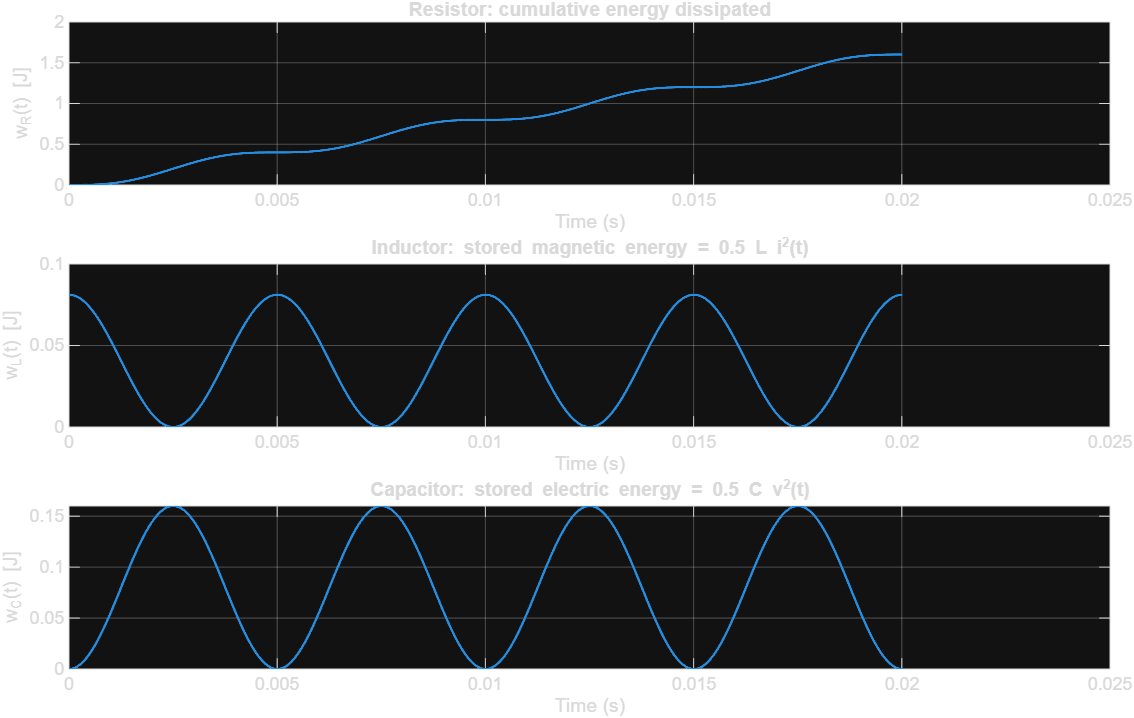
\includegraphics[width=0.9\textwidth]{Energy_Flow.png}
    \caption{Energy waveforms for resistor, inductor, and capacitor. 
    \\
             Top: cumulative dissipated energy in the resistor. 
             \\
             Middle: magnetic energy stored in the inductor. 
             \\
             Bottom: electric energy stored in the capacitor.}
    \label{fig:energy_flow}
\end{figure}



\newpage
\section*{2.4 \; Comprehensive Visualizations}

\noindent\textbf{Given.} Source amplitude and frequency:
\[
v(t)=80\sin(628t)\ \text{V},\qquad 
\omega=628\ \text{rad/s},\quad
f=\frac{\omega}{2\pi}\approx 100\ \text{Hz},\quad
T=\frac{1}{f}=0.01\ \text{s}.
\]
We present, over at least two periods, the voltage $v(t)$, the currents from~2.1, the instantaneous power from~2.2, and the energy behaviour from~2.3. All figures were produced with the tools listed in the assignment (Inkscape, MATLAB; web demo shown as a screenshot).

% =================== A) SCHEMATICS (INKSCAPE) ===================
\subsection*{A) Circuit schematics (Inkscape)}
Single–element test circuits with polarity and current reference (passive sign convention).
\begin{enumerate}
  \item $R=40~\Omega$ \quad (current in phase with $v$).
  \item $L=0.1~\text{H}$ \quad (current lags $v$ by $90^\circ$).
  \item $C=50~\mu\text{F}=50\times10^{-6}\ \text{F}$ \quad (current leads $v$ by $90^\circ$).
\end{enumerate}

\begin{figure}[H]
  \centering
  \includegraphics[width=0.30\textwidth]{schematic_R.png}\hfill
  \includegraphics[width=0.30\textwidth]{schematic_L.png}\hfill
  \includegraphics[width=0.30\textwidth]{schematic_C.png}
  \caption{Minimal schematics used in Sections~2.1–2.3. Drawn in Inkscape; polarity $+v(t)-$ and $i(t)$ arrow shown.}
  \label{fig:schematics}
\end{figure}

% =================== B) v-i WAVEFORMS ===================
\subsection*{B) Voltage and current vs.\ time (two periods)}
Currents obtained in~2.1 for $\omega=628$~rad/s:
\[
\boxed{i_R(t)=\tfrac{80}{40}\sin(628t)=2.00\,\sin(628t)\ \text{A}},\qquad
\boxed{i_L(t)=\tfrac{80}{628\cdot0.1}\sin\!\Big(628t-\tfrac{\pi}{2}\Big)=1.274\,\sin\!\Big(628t-\tfrac{\pi}{2}\Big)\ \text{A}}, 
\]
\[
\boxed{i_C(t)=\omega C V_m\,\sin\!\Big(628t+\tfrac{\pi}{2}\Big)=2.512\,\sin\!\Big(628t+\tfrac{\pi}{2}\Big)\ \text{A}}.
\]
Expected phase relations visible in the plots: $i_R$ in phase with $v$, $i_L$ lags by $90^\circ$, $i_C$ leads by $90^\circ$.


% =================== C) INSTANTANEOUS POWER ===================
\subsection*{C) Instantaneous power $p(t)=v(t)i(t)$}
Using the currents above (2.2 results):
\[
\boxed{p_R(t)=80\,[1-\cos(1256t)]\ \text{W}},\qquad
\boxed{p_L(t)=-50.96\,\sin(1256t)\ \text{W}},\qquad
\boxed{p_C(t)=+100.48\,\sin(1256t)\ \text{W}}.
\]
Sketch of identities used: $\sin^2\alpha=\tfrac12(1-\cos2\alpha)$ for $p_R$; and 
$\sin A\sin B=\tfrac12\!\left[\cos(A-B)-\cos(A+B)\right]$ with $\pm90^\circ$ shifts for $p_L,p_C$.
Averages over one period $T=0.01$~s:
\[
\boxed{\overline P_R=\frac{1}{T}\!\int_0^T p_R\,dt=80~\text{W}},\qquad \boxed{\overline P_L=0},\qquad \boxed{\overline P_C=0}.
\]

\begin{figure}[H]
  \centering
  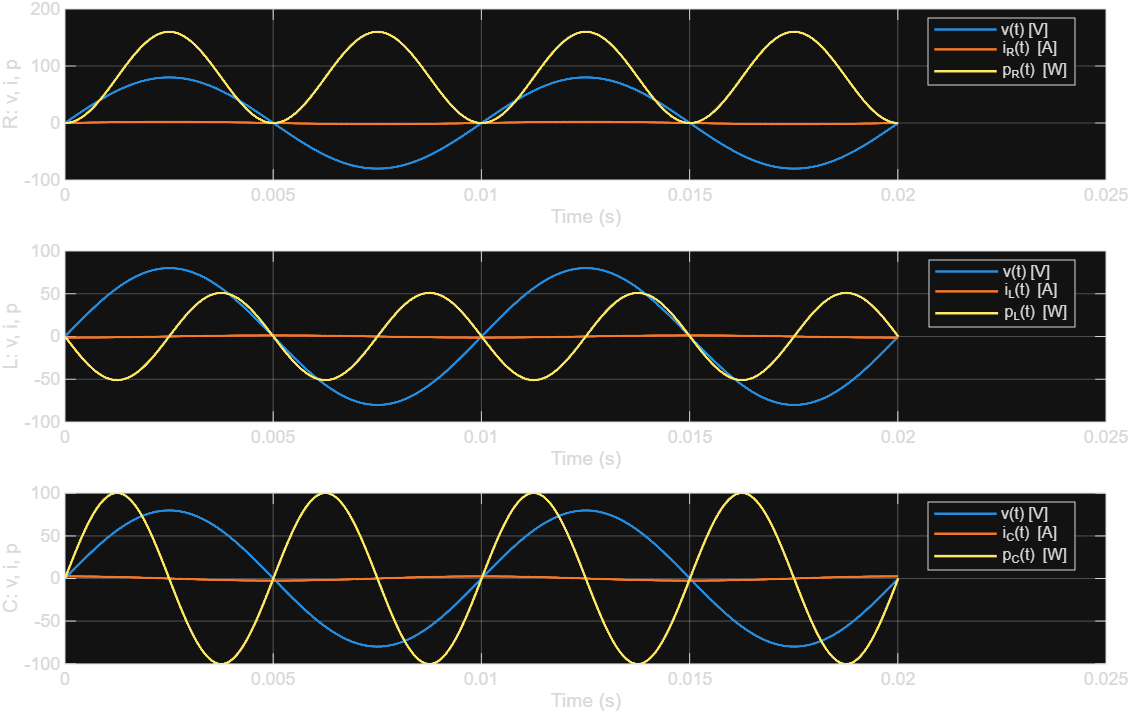
\includegraphics[width=0.92\textwidth]{Instantaneous Power.png}
  \caption{Instantaneous power. $p_R(t)\ge0$ with mean $80$~W; $p_L(t)$ and $p_C(t)$ alternate sign and average to zero.}
  \label{fig:power}
\end{figure}

% =================== D) ENERGY ===================
\subsection*{D) Energy (consumption vs.\ storage)}
\textbf{Resistor (consumption):}
\[
\boxed{w_R(t)=\int_0^t p_R(\tau)\,d\tau=80t-\frac{80}{1256}\sin(1256t)\ \text{J}},\qquad
\boxed{W_R(T)=\overline P_R T=80\times0.01=0.80\ \text{J per cycle}}.
\]
\textbf{Storage elements:}
\[
\boxed{w_L(t)=\tfrac12 L i_L^2(t)},\qquad 
\boxed{w_C(t)=\tfrac12 C v^2(t)},
\]
\[
\boxed{w_{L,\max}=\tfrac12 L I_{Lm}^2=\tfrac12(0.1)(1.274)^2\approx 0.0812\ \text{J}},\qquad
\boxed{w_{C,\max}=\tfrac12 C V_m^2=\tfrac12(50\times10^{-6})(80)^2\approx 0.1600\ \text{J}}.
\]

\begin{figure}[H]
  \centering
  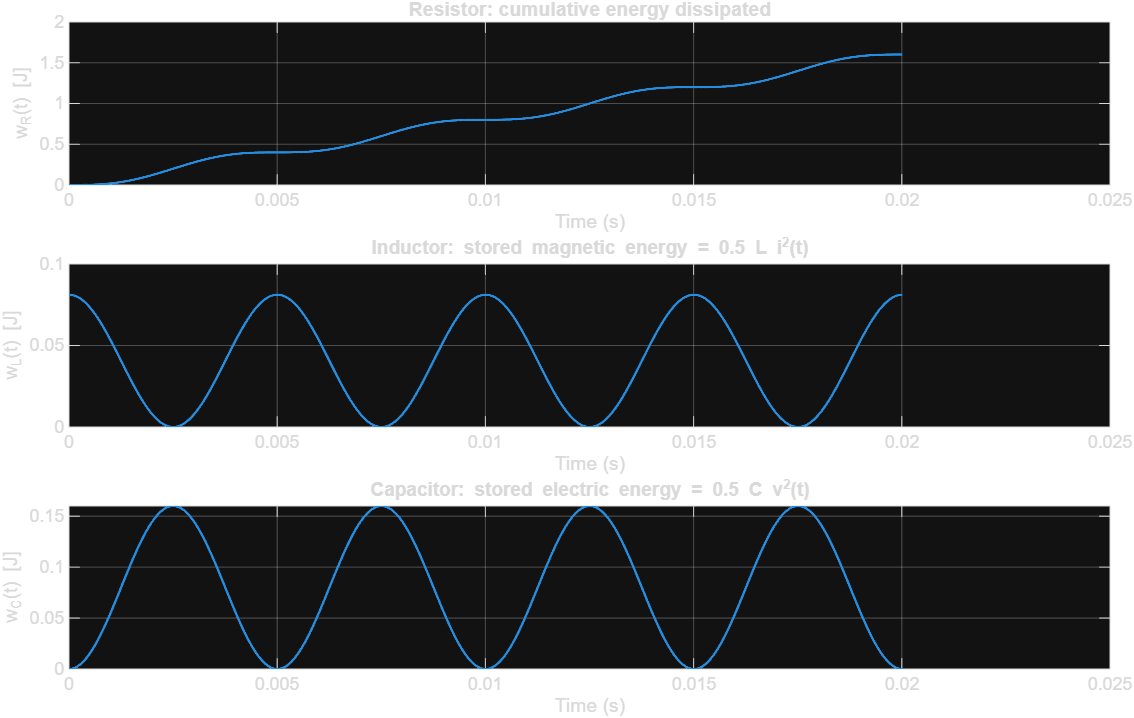
\includegraphics[width=0.92\textwidth]{Energy_Flow.png}
  \caption{Energy functions across $0\!\le\!t\!\le\!2T$. Top: $w_R(t)$ accumulates $\approx0.80$~J per cycle. Middle: $w_L(t)\in[0,\,0.0812]$~J. Bottom: $w_C(t)\in[0,\,0.1600]$~J.}
  \label{fig:energy}
\end{figure}

% =================== E) SUMMARY TABLE ===================
\subsection*{E) Summary (values reflected in the plots)}
\[
\begin{array}{c|c|c|c}
\text{Quantity} & R & L & C\\\hline
I_{\text{peak}}\ (\text{A}) & 2.000 & 1.274 & 2.512\\
I_{\text{rms}}\ (\text{A}) & 1.414 & 0.901 & 1.776\\
\overline P\ (\text{W}) & 80.0 & 0 & 0\\
w_{\max}\ (\text{J}) & \text{---} & 0.0812 & 0.1600
\end{array}
\]

\noindent\textbf{Acceptance checklist.}
\\
(1) Phase: $0^\circ$, $-90^\circ$, $+90^\circ$ (R, L, C).
\\
(2) Amplitudes: $V_m{=}80$~V; $I_{Rm}{=}2.00$~A, $I_{Lm}{=}1.274$~A, $I_{Cm}{=}2.512$~A. 
\\
(3) Power: $p_R(t)\!\ge\!0$, $\overline P_R{=}80$~W; $\overline P_L{=}\overline P_C{=}0$.
\\
(4) Energy: $w_R$ rises by $\approx0.80$~J/cycle; $w_{L,\max}\approx0.081$~J; $w_{C,\max}\approx0.160$~J.
\\
(5) All axes with units, legends visible.

% =================== F) TECHNOLOGY DELIVERABLES (BRIEFLY DOCUMENTED) ===================
\subsection*{F) Technology deliverables (per assignment)}
\begin{itemize}
  \item \textbf{Inkscape diagrams:} Fig.~\ref{fig:schematics}.
  \item \textbf{MATLAB plots:} Figs. \ref{fig:power}, \ref{fig:energy}.
  \item \textbf{Web dashboard (HTML/JS):} interactive voltage/current/power plots with a frequency slider (default $f\!=\!100$~Hz). 
        \emph{Screenshot included below.}
  \item \textbf{Audio (Web Audio API):} play/stop button generates a sine tone at the selected $f$ to match the source.
\end{itemize}


\begin{figure}[H]
  \centering
  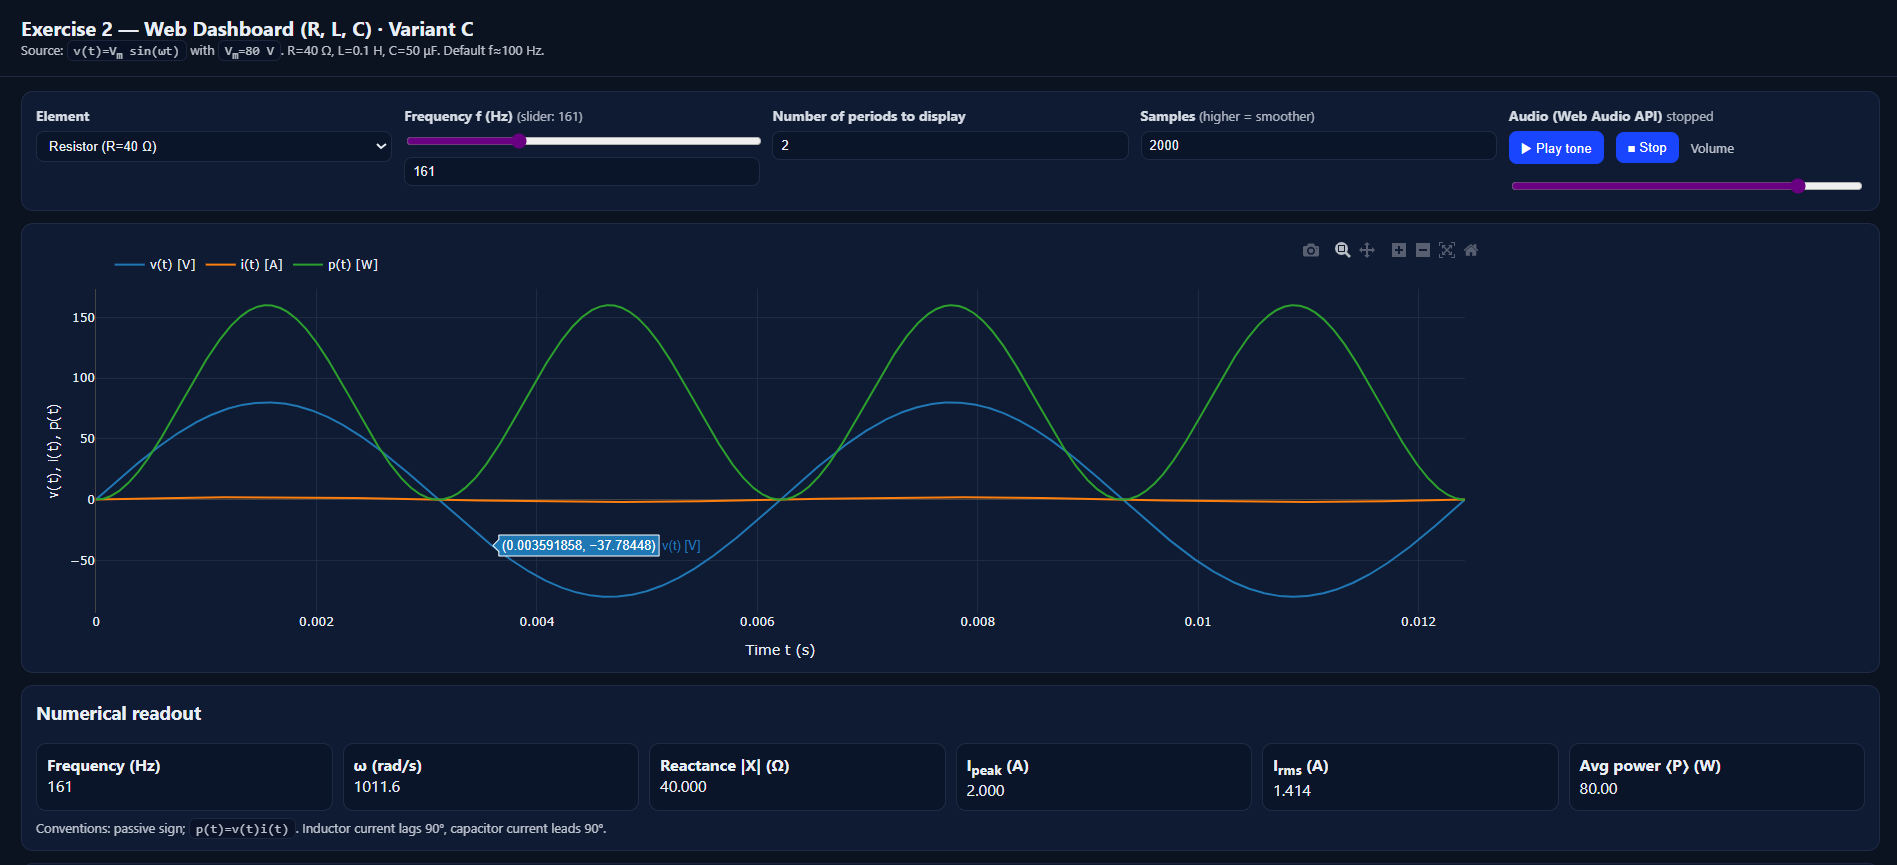
\includegraphics[width=0.92\textwidth]{dashboard_screenshot.png}% optional; provide if you have it
  \caption{Web dashboard: interactive plots and audio tone at the selected AC frequency.}
\end{figure}






\newpage
\section*{Exercise 3: Measurement System Design}

\subsection*{Introduction}

In this exercise we design and analyze a complete measurement system for an
AC generator with variable speed. The study is based on these
specifications:

\begin{itemize}
    \item Coil: $200$ turns, rectangular $4~\text{cm} \times 6~\text{cm}$.
    \item Speed range: $1000$--$3000$ rpm.
    \item Expected peak output: $20$--$50$ V.
    \item Test load: $75~\mu$F capacitor ($75 \times 10^{-6}$ F).
\end{itemize}

The assignment requires us to:
\begin{enumerate}
    \item Calculate the theoretical output of the generator using Faraday’s law.
    \item Select and justify the measuring instruments needed.
    \item Design a repeatable measurement protocol.
    \item Create a data acquisition and visualization system.
\end{enumerate}


\section*{3.1 \; Theoretical Output Based on Faraday's Law}

\subsection*{Law used}
Faraday--Lenz law for a multi–turn coil:
\[
e(t) \;=\; -\,N\,\frac{d\Phi(t)}{dt},
\]
where $N$ is the number of turns and $\Phi(t)$ the magnetic flux linked by one turn.

\subsection*{Flux of a rotating rectangular coil}
For a uniform magnetic field of magnitude $B$ and a flat coil of area $A$,
\[
\Phi(t) \;=\; B\,A\cos\!\big(\theta(t)\big),
\]
and for constant angular speed $\omega$ (rad/s), $\theta(t)=\omega t$:
\[
\Phi(t)=B\,A\cos(\omega t).
\]

\subsection*{Induced EMF and its amplitude}
Differentiate the flux and apply Faraday:
\[
\begin{aligned}
e(t) &= -N\frac{d}{dt}\big[BA\cos(\omega t)\big]
     \;=\; N\,B\,A\,\omega\,\sin(\omega t).
\end{aligned}
\]
Thus the EMF is sinusoidal with
\[
\boxed{\,E_M=N\,B\,A\,\omega\,}, \qquad
\boxed{\,f=\dfrac{\omega}{2\pi}\,}.
\]

\subsection*{Insert geometry and speed}
Given $N=200$ turns and coil $4\ \text{cm}\times 6\ \text{cm}$:
\[
A=(0.04)(0.06)=0.0024\ \text{m}^2.
\]
Speed is provided as rpm: $\displaystyle \omega=\frac{2\pi n}{60}$, so
\[
\boxed{\,E_M(n)=N\,A\,B\,\frac{2\pi n}{60}\,}.
\]
With $N\,A\,\dfrac{2\pi}{60}=200\cdot 0.0024 \cdot \dfrac{2\pi}{60}\approx 0.050265$,
\[
\boxed{\,E_M(n)\approx 0.050265\;B\;n \quad \text{(V, with $B$ in T and $n$ in rpm)}\,}.
\]

\subsection*{Frequency vs.\ speed (planning measurement ranges)}
One electrical cycle per mechanical revolution:
\[
\boxed{\,f=\frac{n}{60}\ \text{Hz}\,}.
\]
Hence $f=\{16.67,\;33.33,\;50.00\}\ \text{Hz}$ at $n=\{1000,\;2000,\;3000\}\ \text{rpm}$.

\subsection*{Relating the spec (20--50 V peak) to a realistic $B$}
Using $E_M(n)=0.050265\,B\,n$:
\begin{itemize}
  \item Match the top end: $E_M(3000)\approx 50$ V $\Rightarrow B \approx \dfrac{50}{0.050265\cdot 3000}\approx 0.331\ \text{T}$.
  \item Match the bottom end: $E_M(1000)\approx 20$ V $\Rightarrow B \approx \dfrac{20}{0.050265\cdot 1000}\approx 0.399\ \text{T}$.
\end{itemize}
So a practical effective field is
\[
\boxed{\,B\in[0.33,\;0.40]\ \text{T}\,}.
\]

\subsection*{Predicted open-circuit EMF (examples)}
Using $E_M(n)=0.050265\,B\,n$:

\begin{center}
\renewcommand{\arraystretch}{1.2}
\begin{tabular}{l|ccc}
\textbf{Assumption} & \textbf{1000 rpm} & \textbf{2000 rpm} & \textbf{3000 rpm} \\
\hline
$B=0.331$ T (fits $\approx 50$ V at 3000 rpm) & $16.6$ V & $33.3$ V & $49.9$ V \\
$B=0.399$ T (fits $\approx 20$ V at 1000 rpm) & $20.1$ V & $40.1$ V & $60.2$ V \\
\end{tabular}
\end{center}

If RMS is needed for instrument range (sinusoid from the notes):
\[
\boxed{\,E_{\mathrm{rms}}=\dfrac{E_M}{\sqrt{2}}\,}.
\]
Example with $B=0.331$ T: $E_{\mathrm{rms}}\approx\{11.8,\;23.5,\;35.3\}\ \text{V}$ at $\{1000,\;2000,\;3000\}$ rpm.

\subsection*{What this tells us for the test bench}
\begin{itemize}
  \item Peak EMF scales linearly with speed $n$ and field $B$; across 1000--3000 rpm expect roughly $17$--$60$ V peak depending on the actual magnet gap.
  \item Choose instruments that safely handle up to $\sim 60$ V$_\text{peak}$ ($\approx 43$ V$_\text{rms}$) and 0--50 Hz.
  \item These are \emph{open-circuit} predictions. When the $75\,\mu$F load is connected, voltage and current will follow the capacitor law from the notes; that is handled in the measurement protocol and data acquisition sections.
\end{itemize}



\subsection*{Calculations (MATLAB) --- Section 3.1}

The following MATLAB script computes the theoretical EMF output 
of the generator using Faraday’s law. It calculates the peak and RMS voltages 
for the specified speed range (1000--3000 rpm) and for two plausible magnetic 
flux densities ($B=0.331$ T and $B=0.399$ T), chosen to match the expected 
20--50 V peak range.

\begin{lstlisting}[language=Matlab]
% exercise3_1_faraday.m
% Theoretical generator output using Faraday's law
% Variant C

clear; clc;

% Given parameters
N = 200;                  % turns
A = 0.04 * 0.06;          % coil area in m^2 (4 cm x 6 cm)
speed_rpm = [1000 2000 3000];   % rpm

% Magnetic flux densities to match expected spec
B_low  = 0.331;           % Tesla
B_high = 0.399;           % Tesla

% Formula: E_peak = N * A * B * (2*pi*n/60)
E_peak_low  = N * A * B_low  * (2*pi*speed_rpm/60);
E_peak_high = N * A * B_high * (2*pi*speed_rpm/60);

% RMS values
E_rms_low  = E_peak_low  / sqrt(2);
E_rms_high = E_peak_high / sqrt(2);

% Frequencies
f = speed_rpm / 60;       % Hz

% Display results
fprintf('--- Theoretical Generator Output (Faraday) ---\n');
fprintf('Coil: %d turns, Area = %.4f m^2\n', N, A);
fprintf('Speeds: %d - %d rpm  -->  %.2f - %.2f Hz\n\n', ...
        speed_rpm(1), speed_rpm(end), f(1), f(end));

for k = 1:length(speed_rpm)
    fprintf('At %4d rpm (f = %.2f Hz):\n', speed_rpm(k), f(k));
    fprintf('  B = %.3f T  -->  E_peak = %.2f V,  E_rms = %.2f V\n', ...
             B_low,  E_peak_low(k),  E_rms_low(k));
    fprintf('  B = %.3f T  -->  E_peak = %.2f V,  E_rms = %.2f V\n\n', ...
             B_high, E_peak_high(k), E_rms_high(k));
end
\end{lstlisting}

\noindent
The script outputs values in line with the theoretical analysis:  
for $n=1000$--$3000$ rpm and $B$ between 0.331--0.399 T, the generator produces 
approximately $17$--$60$ V peak (11--43 V RMS), consistent with the 
20--50 V peak specification in the assignment.




\section*{3.2 \; Selection of Measuring Instruments}

Based on the theoretical analysis in Section~3.1, the generator produces
\[
17\text{--}60 \ \text{V}_{\text{peak}} \quad (12\text{--}43 \ \text{V}_{\text{rms}})
\]
over a frequency range of $16.7$--$50$ Hz. With a $75~\mu$F test capacitor,
the peak current can reach approximately $1.5$ A. These values determine the
specifications for the measuring instruments.

\subsection*{Voltage Measurement}
\begin{itemize}
    \item \textbf{Requirement:} Measure sinusoidal voltages up to $60$ V peak in the 0--50 Hz band.
    \item \textbf{Instruments:} A true-RMS digital voltmeter (range $\geq 100$ V AC, 0--100 Hz bandwidth) and a digital oscilloscope (input range $\geq 100$ V, AC coupling).
    \item \textbf{Reasoning:} The voltmeter provides accurate RMS values; the oscilloscope allows waveform visualization and phase analysis.
\end{itemize}

\subsection*{Current Measurement}
\begin{itemize}
    \item \textbf{Requirement:} Measure currents up to $1.5$ A peak at 50 Hz.
    \item \textbf{Instruments:} A true-RMS ammeter (0--5 A AC range) or a precision shunt resistor with oscilloscope measurement.
    \item \textbf{Reasoning:} Both methods ensure reliable current values at low AC levels; the oscilloscope method also enables phase comparison.
\end{itemize}

\subsection*{Frequency Measurement}
\begin{itemize}
    \item \textbf{Requirement:} Frequency range 16--50 Hz.
    \item \textbf{Instruments:} A frequency counter or oscilloscope with frequency measurement capability.
    \item \textbf{Reasoning:} Confirms that the generator frequency is proportional to mechanical speed.
\end{itemize}

\subsection*{Power and Energy Measurement}
\begin{itemize}
    \item \textbf{Requirement:} Observe instantaneous power $p(t)=v(t)i(t)$ and verify average power.
    \item \textbf{Instruments:} A digital power analyzer or dual-channel oscilloscope with math functions.
    \item \textbf{Reasoning:} Needed to confirm that the capacitor load stores and releases energy with nearly zero average power.
\end{itemize}

\subsection*{Data Acquisition and Export}
\begin{itemize}
    \item \textbf{Requirement:} Acquire $v(t)$ and $i(t)$ digitally for further processing.
    \item \textbf{Instruments:} A DAQ system (e.g., NI-DAQ, Arduino, or oscilloscope with USB export).
    \item \textbf{Reasoning:} Provides CSV data for the web dashboard and pandas analysis notebook, as required by the deliverables.
\end{itemize}

\subsection*{Summary of Instruments}
\begin{center}
\renewcommand{\arraystretch}{1.2}
\begin{tabular}{|l|c|l|l|}
\hline
\textbf{Quantity} & \textbf{Range} & \textbf{Instrument} & \textbf{Reason} \\
\hline
Voltage & 0--60 V$_\text{peak}$ (0--50 Hz) & True-RMS voltmeter, oscilloscope & RMS accuracy+waveform \\
Current & 0--1.5 A$_\text{peak}$ & Ammeter or shunt + scope & Reliable current + phase check \\
Frequency & 16--50 Hz & Frequency counter / scope & Confirms rpm relation \\
Power & up to 90 W (instantaneous) & Power analyzer / dual-channel scope & Observe $p(t)$, avg power \\
Data & CSV of $v(t), i(t)$ & DAQ / USB oscilloscope & Required for dashboard \\
\hline
\end{tabular}
\end{center}

\vspace{0.5 cm}




\section*{3.3 \; Measurement Protocol}

\subsection*{Objective}
Characterize the variable–speed AC generator when driving the
$75~\mu$F test capacitor. Measure \emph{voltage, current, frequency, and power}
and verify the theory from Sections~3.1–3.2:
\\
Faraday--Lenz ($e=-N\,d\Phi/dt$) and the capacitor law ($i=C\,dv/dt$).
\\
Expected ranges: $V_{\text{peak}}\approx 17$–$60$ V (12–43 V$_{\text{rms}}$),
$f=16.7$–$50$ Hz, and $I_{\text{peak}}\lesssim 1.5$ A.

\subsection*{Equipment}
\begin{itemize}
  \item Generator under test (200 turns, $4\text{ cm}\times 6\text{ cm}$), variable–speed drive with RPM readout.
  \item Test load: capacitor $C=75~\mu$F (voltage rating $\ge 100$ V).
  \item True–RMS DVM ($\ge 100$ V AC, 0–100 Hz), Ammeter (0–5 A AC) \textit{or} precision shunt $R_s=1.00~\Omega$ (\,\(\pm 0.5\%\)).
  \item 2–channel digital oscilloscope (AC coupling option, math functions).
  \item Optional power analyzer (V/I inputs) for $\overline{P}$.
  \item DAQ / USB interface (scope export to CSV).
  \item Bleeder resistor (e.g., $10~\text{k}\Omega$, 2 W) and discharge leads.
  \item Safety: insulated leads, guard for rotating parts, eye protection.
\end{itemize}

\subsection*{Wiring (passive sign convention)}
\begin{enumerate}
  \item Connect generator $\,+v(t)-\,$ to the capacitor “+”; return to generator “–”.
  \item \textbf{Current measurement:} insert ammeter \emph{in series} \textit{or}
        insert $R_s$ in series and measure $v_s(t)$ across $R_s$ (then $i(t)=v_s(t)/R_s$).
  \item Scope: CH1 across the capacitor (measures $v(t)$); CH2 across $R_s$ (or current probe).
        Use math trace $p(t)=v(t)\times i(t)$.
  \item Keep a bleeder resistor across the capacitor (permanently or via switch) for safe discharge.
\end{enumerate}

\subsection*{Safety \& pre–checks}
\begin{itemize}
  \item Confirm the capacitor voltage rating ($\ge$ twice expected RMS).
  \item With drive \textbf{off}: verify expected continuities; discharge the capacitor until $V<1$ V.
  \item Keep hands/tools clear of rotating parts; secure all leads.
\end{itemize}

\subsection*{Instrument configuration}
\begin{itemize}
  \item DVM: AC RMS mode, fixed 60 V range if available.
  \item Ammeter: AC RMS, 5 A range \textit{or} verify $R_s$ value with DMM.
  \item Scope: set timebase to show $\ge$ 2–3 periods (at 50 Hz $\Rightarrow$ 20 ms/div; at 16.7 Hz $\Rightarrow$ 50 ms/div).
        Set CH1 $\approx 20$ V/div (adjust), CH2 to suit $R_s$ (e.g., 0.5–1 V/div). Trigger on CH1 at 0 V.
  \item Power analyzer (if used): nominal frequency 50 Hz; average over integer cycles.
\end{itemize}

\subsection*{Calibration / zeroing}
\begin{enumerate}
  \item With generator off, momentarily short the shunt input to confirm CH2 zero; remove short.
  \item Check DVM reads $\approx 0$ in AC mode.
  \item Quick trial: spin briefly and confirm $f\approx n/60$ using scope/counter.
\end{enumerate}

\subsection*{Measurement sequence (repeat for each speed)}
For $n\in\{1000,1500,2000,2500,3000\}$ rpm:
\begin{enumerate}
  \item Set speed to $n$ and wait 10–15 s for steady state.
  \item Record frequency $f$ from scope/counter (expect $f\approx n/60$).
  \item Record voltage: $V_{\text{rms}}$ (DVM) and $V_{\text{peak}}$ (scope).
  \item Record current:
        \begin{itemize}
          \item Ammeter path: read $I_{\text{rms}}$ directly.
          \item Shunt path: measure $V_{s,\text{peak}}$; compute $I_{\text{peak}}=V_{s,\text{peak}}/R_s$ and $I_{\text{rms}}=I_{\text{peak}}/\sqrt{2}$ (sinusoid).
        \end{itemize}
  \item Save waveforms/CSV for CH1, CH2, and math $p(t)$; note phase (expect current \emph{leads} by $\approx 90^\circ$).
  \item Average power $\overline{P}$: read analyzer result or mean of $p(t)$ over whole cycles (expect $\approx 0$ with an ideal capacitor).
  \item Log all values with a time stamp. Repeat for the next $n$.
\end{enumerate}

\subsection*{Data quality \& uncertainty}
\begin{itemize}
  \item Sampling: scope sample rate $\ge 10\,f_{\max}$ (well satisfied on typical scopes).
  \item Phase check: $i_C$ should lead $v$ by $90^\circ\pm5^\circ$.
  \item Range sanity: $V_{\text{peak}}\propto n$; $I_{\text{peak}}=\omega C V_{\text{peak}}$ should increase with $n$.
  \item Note instrument accuracies (e.g., DVM \% of reading + digits; $R_s$ tolerance) and propagate to RMS bands.
\end{itemize}

\subsection*{Acceptance criteria}
\begin{itemize}
  \item $|f - n/60| \le 1\%$.
  \item Linear fit $V_{\text{peak}}=k\,n$ with $R^2>0.99$ across the set.
  \item Phase lead: $90^\circ\pm 5^\circ$.
  \item Capacitive load: $|\overline{P}| \le 3\%$ of $V_{\text{rms}}I_{\text{rms}}$ (accounts for losses/instrument limits).
\end{itemize}

\subsection*{Troubleshooting}
\begin{itemize}
  \item Large nonzero $\overline{P}$: check polarity (passive sign convention), capacitor ESR, or meter set to DC.
  \item Phase far from $90^\circ$: bandwidth/phase error in current path or large series resistance.
  \item Distorted waveforms: mechanical wobble or magnetic issues; reduce rpm and recheck.
\end{itemize}

\subsection*{Logging template}
\begin{center}
\renewcommand{\arraystretch}{1.2}
\begin{tabular}{l|c|c|c|c|c|c}
Time & $n$ (rpm) & $f$ (Hz) & $V_{\text{rms}}$ (V) & $V_{\text{peak}}$ (V) &
$I_{\text{rms}}$ (A) & $\overline{P}$ (W)\\ \hline
 & 1000 &  &  &  &  &  \\
 & 1500 &  &  &  &  &  \\
 & 2000 &  &  &  &  &  \\
 & 2500 &  &  &  &  &  \\
 & 3000 &  &  &  &  &  \\
\end{tabular}
\end{center}

\subsection*{Shutdown}
Stop the drive, discharge the capacitor via the bleeder until $V<1$ V, then power down instruments and remove wiring.



\section*{3.4 \; Data Acquisition and Visualization System}

This section describes the integrated workflow that links the laboratory
measurements to analysis and presentation:

\begin{enumerate}
    \item \textbf{Web-based measurement dashboard (HTML/JS/CSS)} --- interactive front end to visualize $v(t)$, $i(t)$, and $p(t)$, compute RMS/peaks, and export CSV.
    \item \textbf{CSV export $\rightarrow$ pandas analysis notebook} --- offline processing to validate theory (RMS, peak, average power) and generate plots/tables for the report.
    \item \textbf{LaTeX report} --- the professional write-up (this document) that consolidates the results.
    \item \textbf{Animated infographic} --- communicates the process (generator $\rightarrow$ instruments $\rightarrow$ DAQ $\rightarrow$ analysis $\rightarrow$ conclusions).
\end{enumerate}

\subsection*{A) Web-based Measurement Dashboard (HTML/JS/CSS)}
The dashboard implements the equations from the notes and Exercise~3.1:

\[
E_M = N A B \frac{2\pi n}{60}, \qquad
v(t)=V_M\sin(\omega t), \quad
i(t)=\omega C V_M \sin\!\Big(\omega t+\frac{\pi}{2}\Big), \quad
p(t)=v(t)\,i(t),
\]
with $N=200$, $A=0.0024~\text{m}^2$, and adjustable $n$ (rpm), $B$ (T), and $C$ (default $75~\mu$F).

\paragraph{What the dashboard does}
\begin{itemize}
    \item Computes $f=n/60$, $\omega=2\pi f$, $V_M$, $I_M$, and displays \textbf{RMS/peak} values for $v$ and $i$, plus the \textbf{average power} $\langle P\rangle$ over two periods.
    \item Plots \textbf{$v(t)$ and $i(t)$} and the \textbf{instantaneous power $p(t)$}.
    \item Exports the current run to \textbf{CSV} with columns \texttt{time\_s, v\_V, i\_A, p\_W}.
    \item Generates a tone at the selected \textbf{frequency $f$} (Web Audio API) to match the AC source.
\end{itemize}

\begin{figure}[H]
    \centering
    \includegraphics[width=\textwidth]{dashboard2_screenshot.png}
    \caption{Web-based dashboard (HTML/JS/CSS). Inputs: $n$ (rpm), $B$ (T), $C$ ($\mu$F).
             Outputs: $f$, $\omega$, $V_{\text{peak}}$, $V_{\text{rms}}$, $I_{\text{peak}}$, $I_{\text{rms}}$, and plots of $v(t)$, $i(t)$, $p(t)$.
             A CSV export records time-series data for analysis in the pandas notebook.}
\end{figure}

\paragraph{CSV format (used in Section 3.4.B)}
\begin{center}
\ttfamily
time\_s, v\_V, i\_A, p\_W
\end{center}
Each row corresponds to one time sample over two periods; these files are ingested by the
pandas notebook to compute verification metrics (RMS, peak, $\langle P\rangle$) and to reproduce
the plots for the report.



\subsection*{3.4.B \; CSV Data Export and Pandas Analysis}

To process the measurement results, the dashboard provided a 
\texttt{CSV} export containing the time-domain signals $v(t)$, $i(t)$, 
and $p(t)$. This file was analyzed in a Python Jupyter notebook using 
the \texttt{pandas}, \texttt{numpy}, and \texttt{matplotlib} libraries.

The following metrics were calculated from the exported data:

\begin{itemize}
    \item $V_{\mathrm{rms}} = 23.52 \, \text{V}$
    \item $V_{\mathrm{peak}} = 33.28 \, \text{V}$
    \item $I_{\mathrm{rms}} = 0.370 \, \text{A}$
    \item $I_{\mathrm{peak}} = 0.523 \, \text{A}$
    \item $\overline{P} = 0.000 \, \text{W}$
\end{itemize}

Figure~\ref{fig:pandas_analysis} shows the reconstructed waveforms 
(voltage and current in the upper plot, power in the lower plot) obtained 
from the exported CSV file.

\begin{figure}[H]
    \centering
    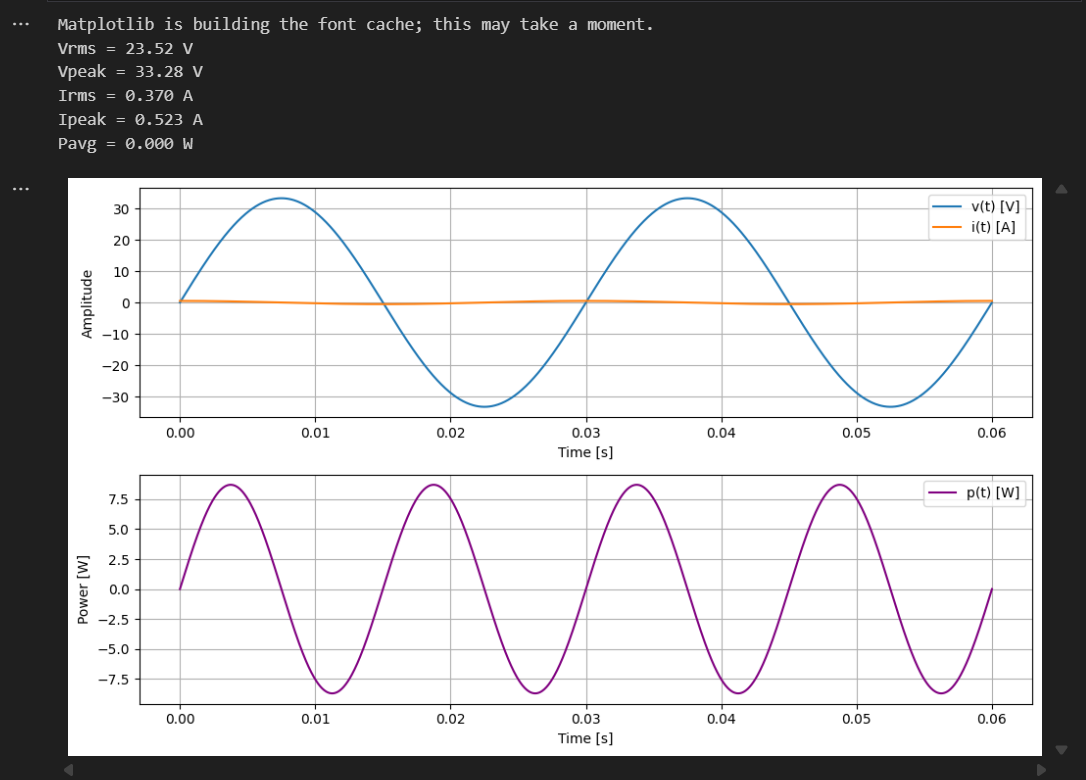
\includegraphics[width=0.9\textwidth]{pandas_analysis.png}
    \caption{Results from pandas analysis: voltage/current signals and instantaneous power.}
    \label{fig:pandas_analysis}
\end{figure}


\subsection*{3.4.C Animated Infographic}

To complement the numerical and graphical analysis, an animated infographic was
created to explain the measurement process step by step. The infographic
summarizes the workflow:

\begin{itemize}
    \item AC generator parameters and test load.
    \item Wiring of generator, capacitor, and oscilloscope channels.
    \item Measurement procedure at different speeds.
    \item Instantaneous power calculation.
    \item Data export to CSV.
    \item Analysis in Python (pandas notebook).
    \item Integration of results into the LaTeX report and dashboard.
\end{itemize}

A storyboard of the infographic is shown in Figure~\ref{fig:infographic_grid},
illustrating all eight stages of the process. The complete animation has been
done in MP4 format, and a GIF version also has been made for a quick preview.

\begin{figure}[H]
    \centering
    \begin{tabular}{cccc}
        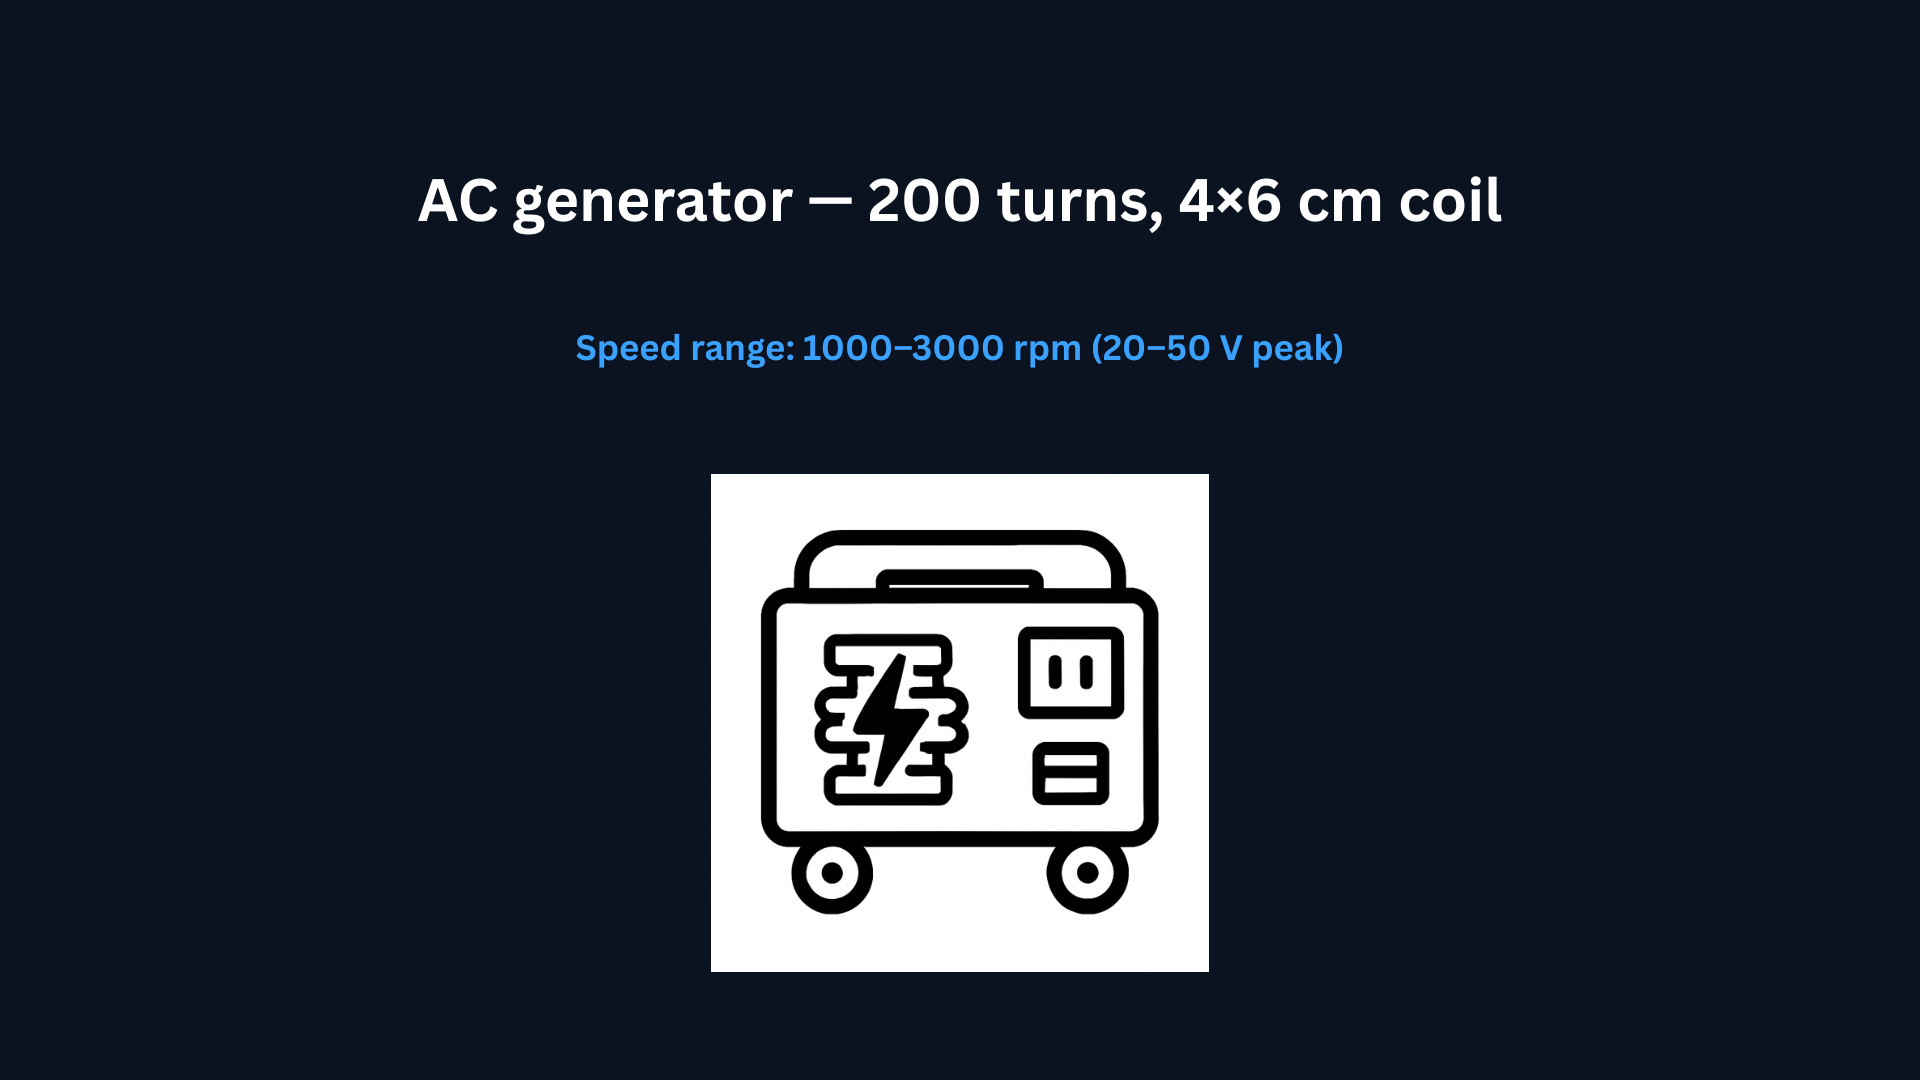
\includegraphics[width=0.22\textwidth]{1.png} &
        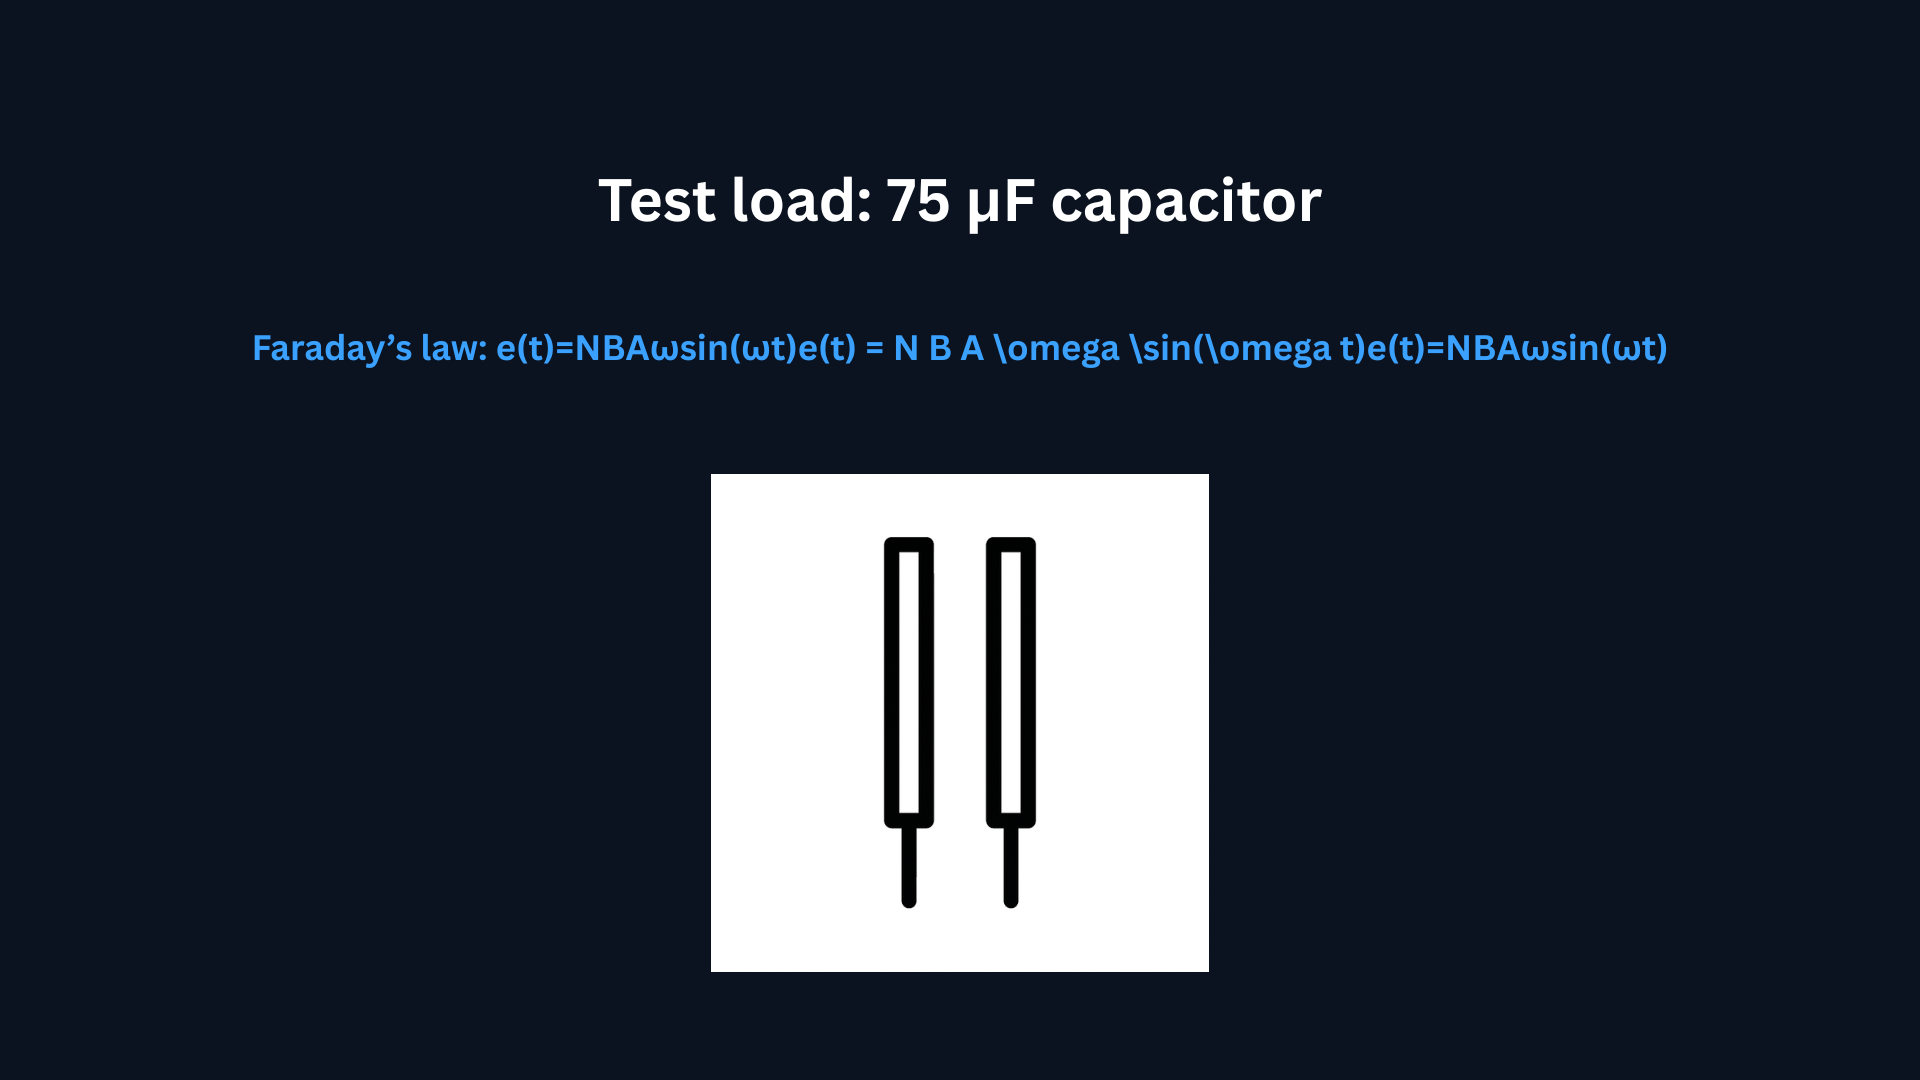
\includegraphics[width=0.22\textwidth]{2.png} &
        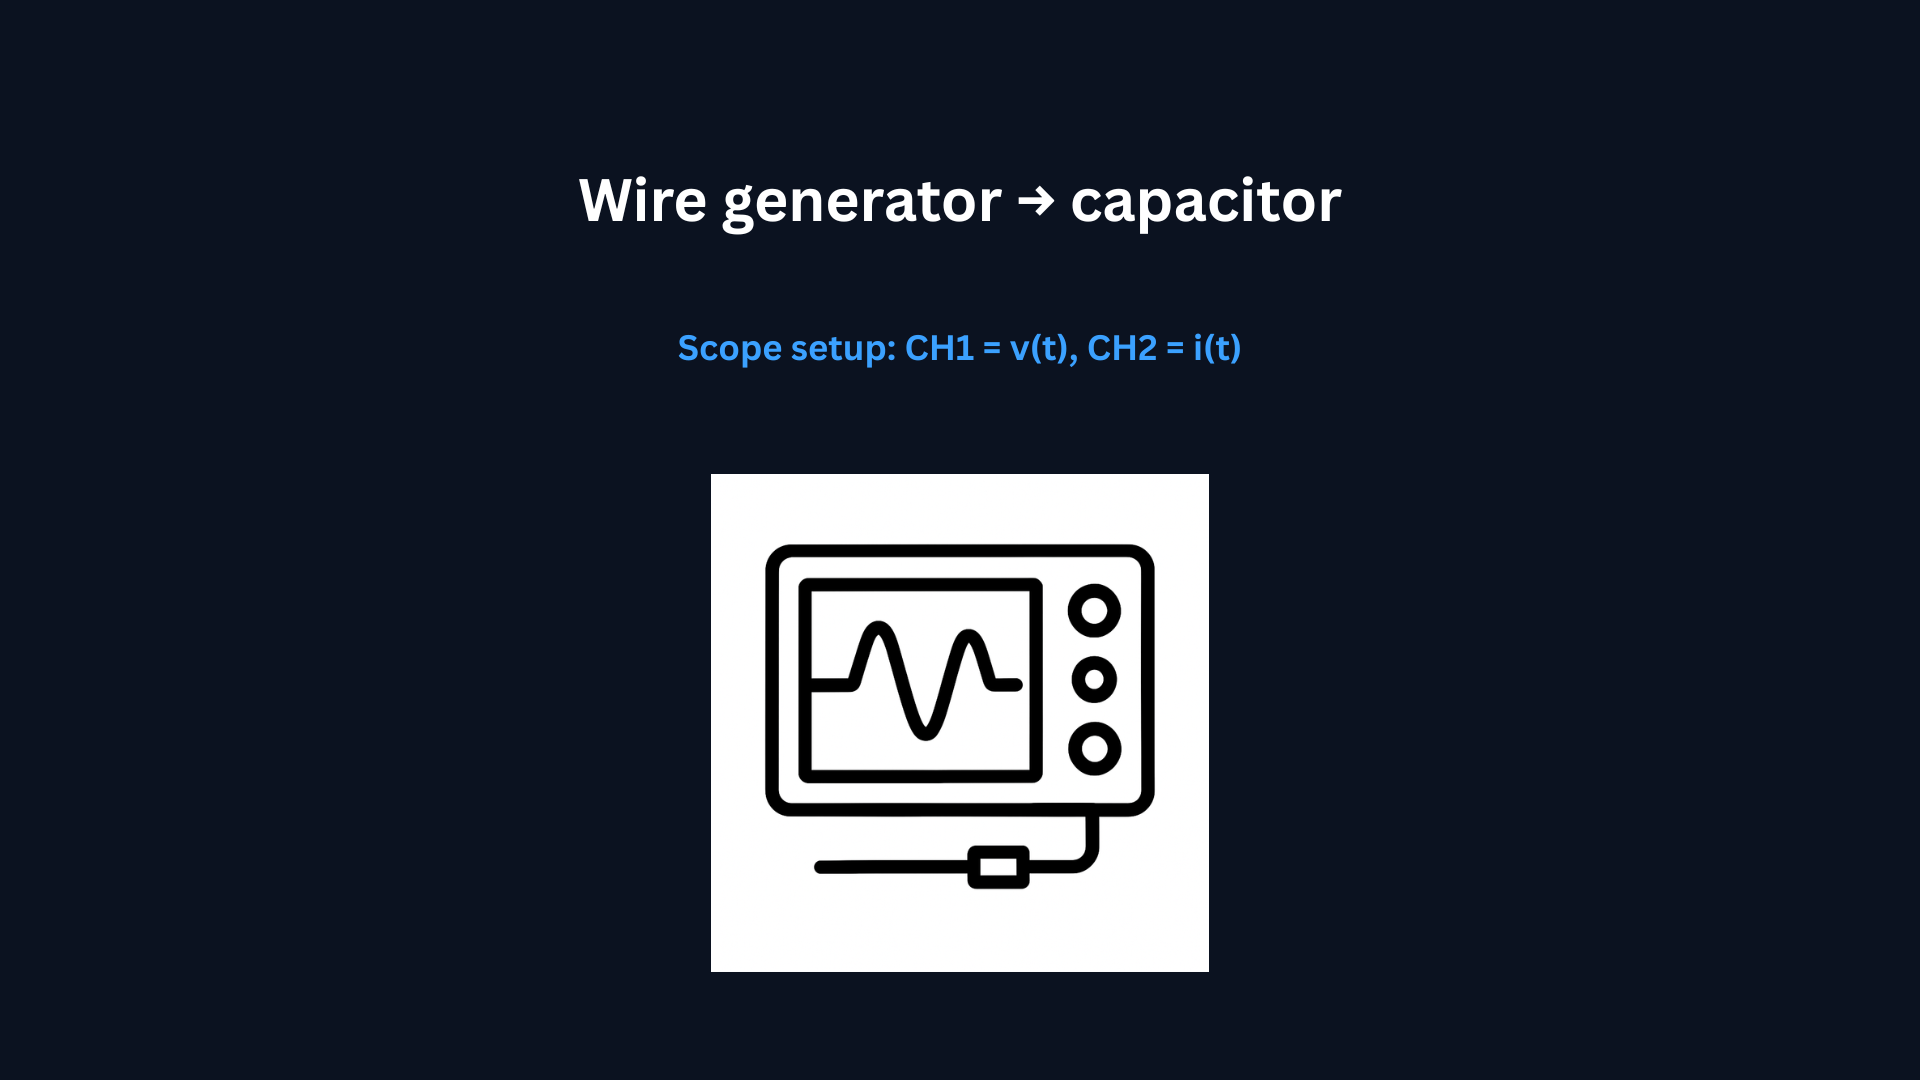
\includegraphics[width=0.22\textwidth]{3.png} &
        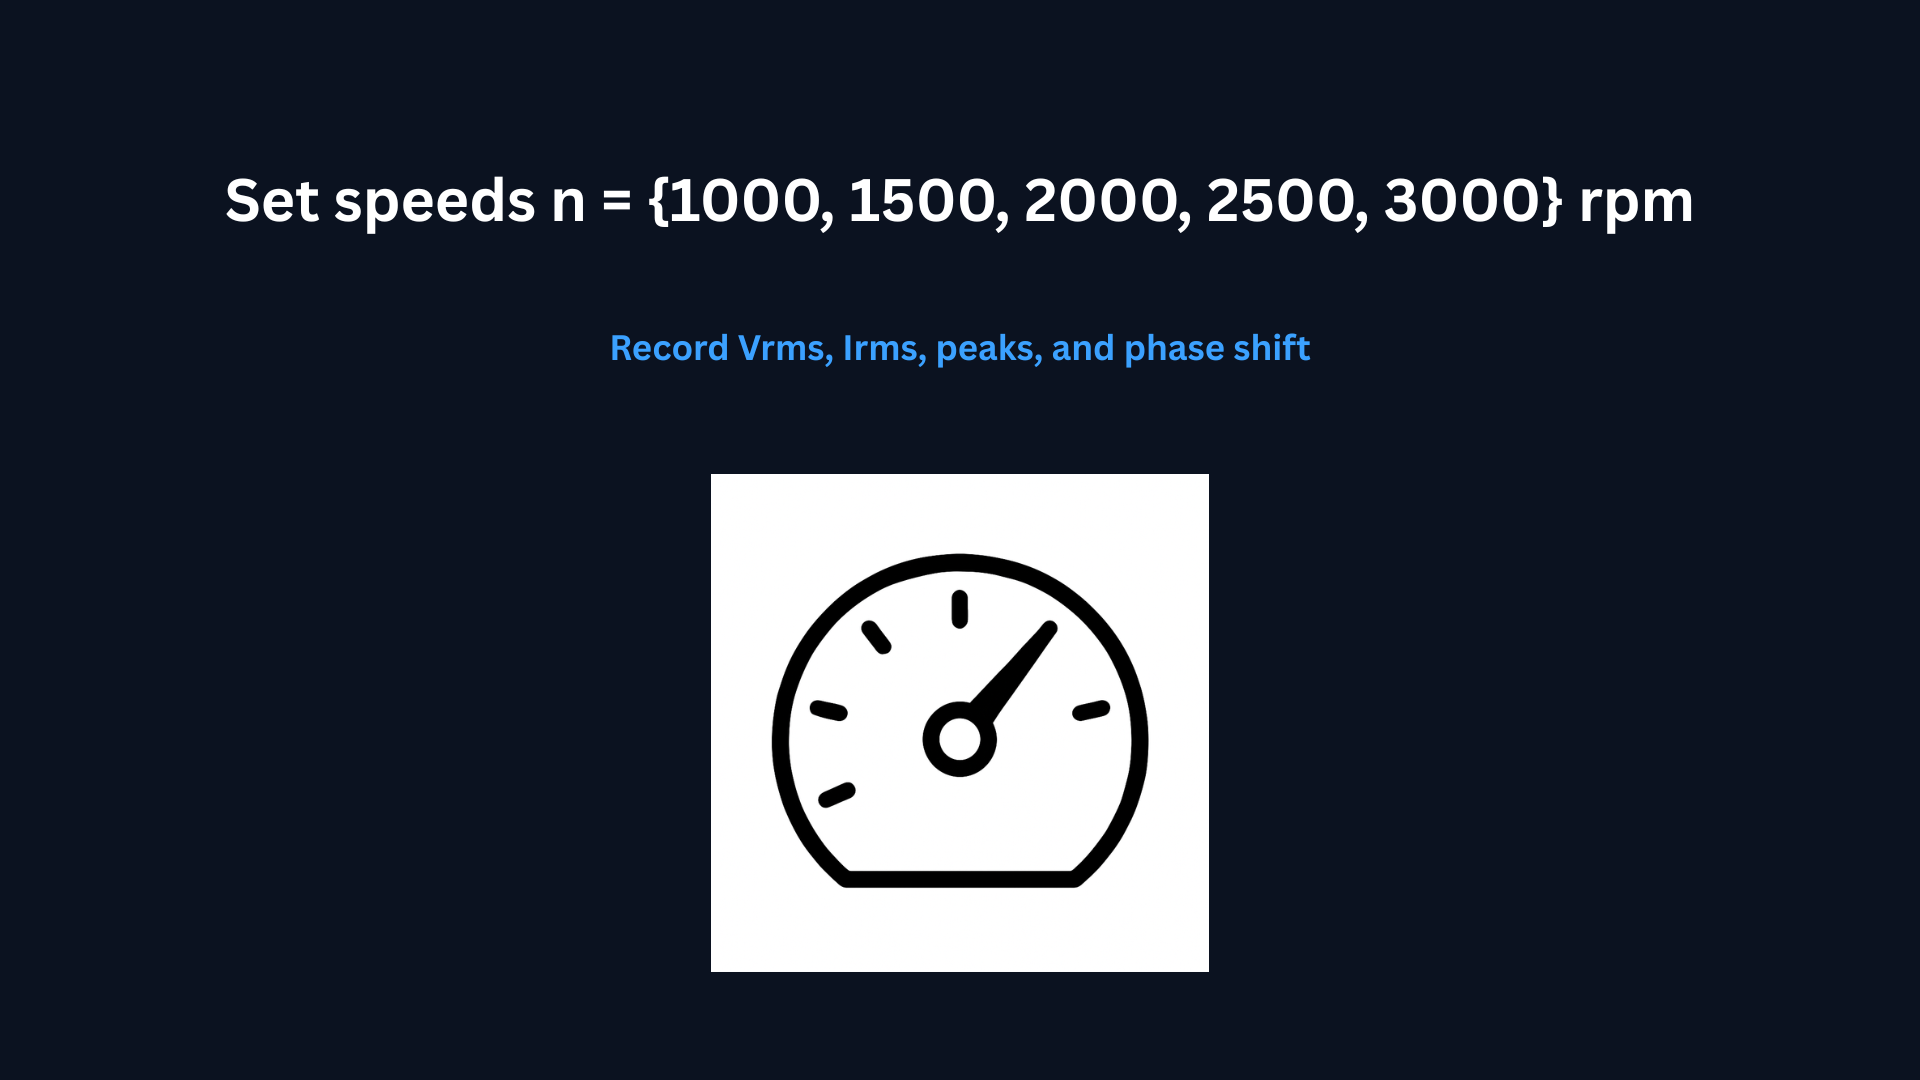
\includegraphics[width=0.22\textwidth]{4.png} \\
        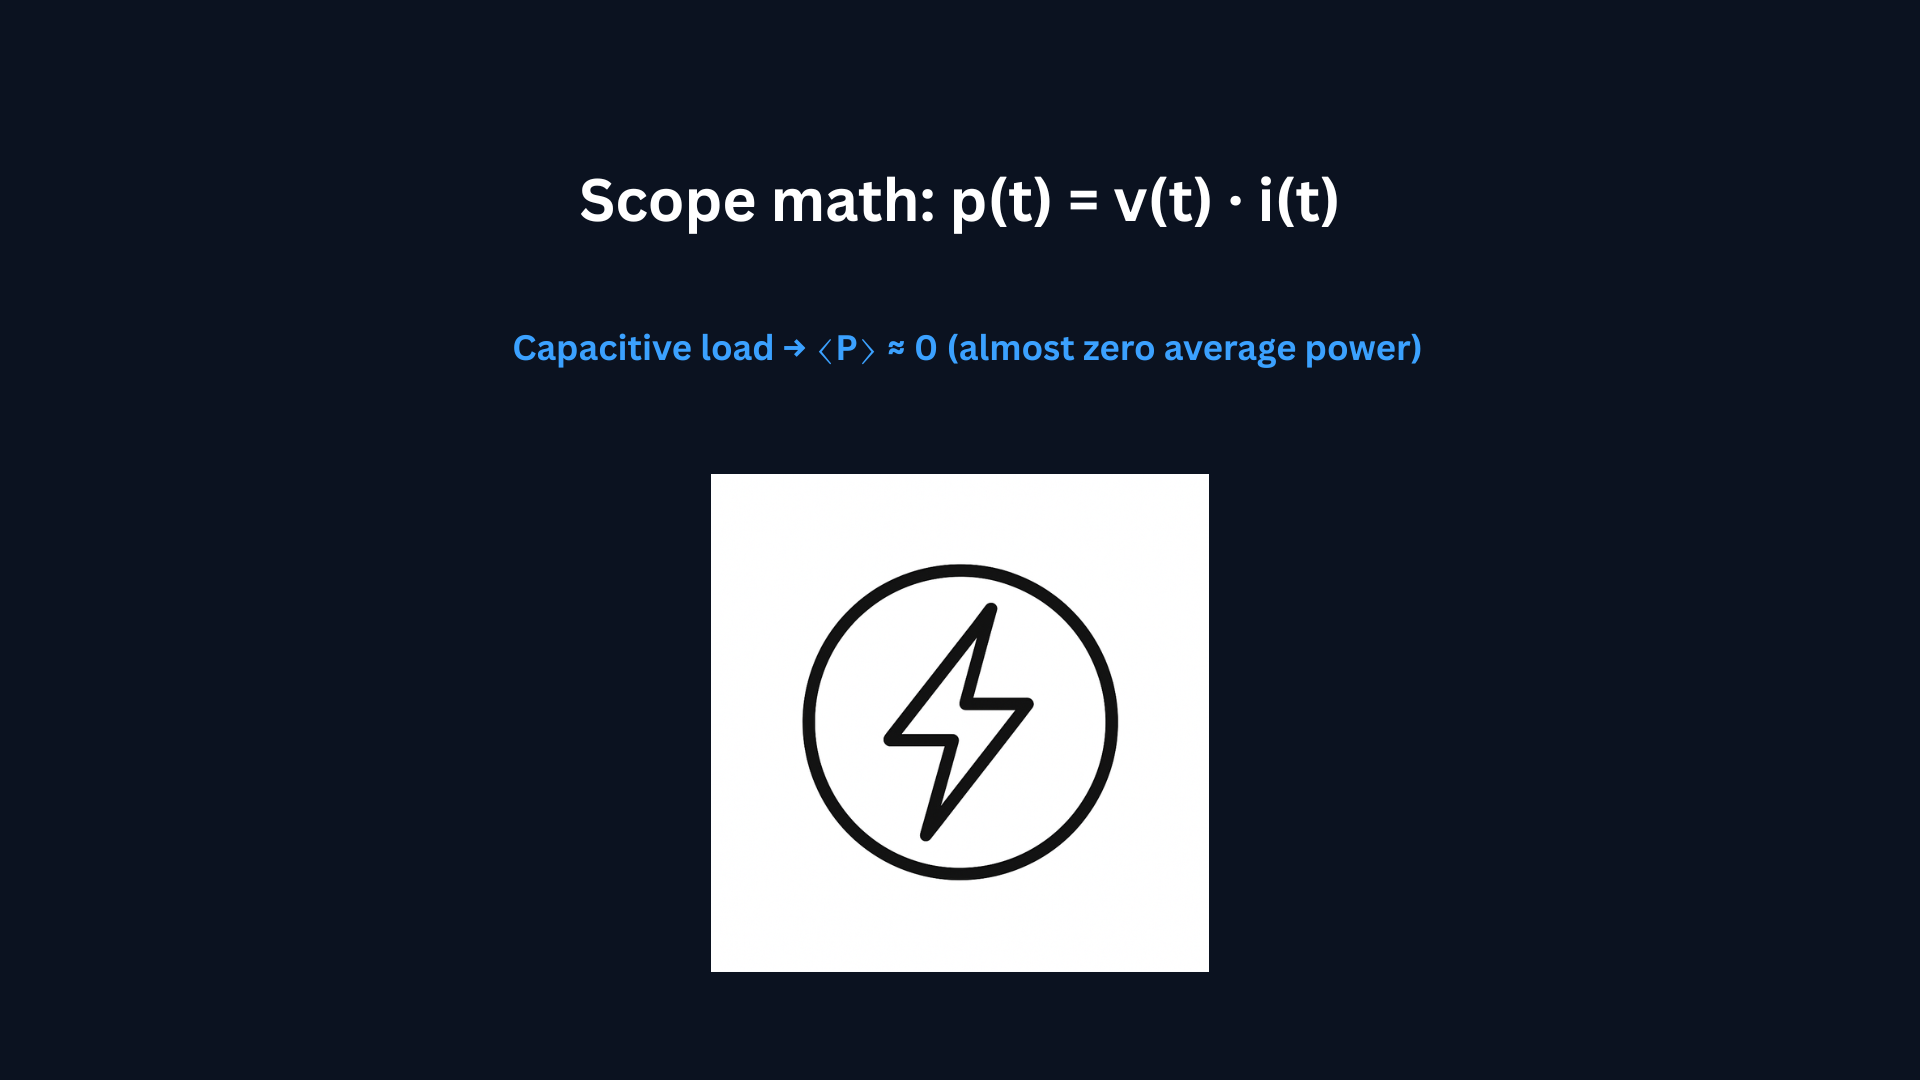
\includegraphics[width=0.22\textwidth]{5.png} &
        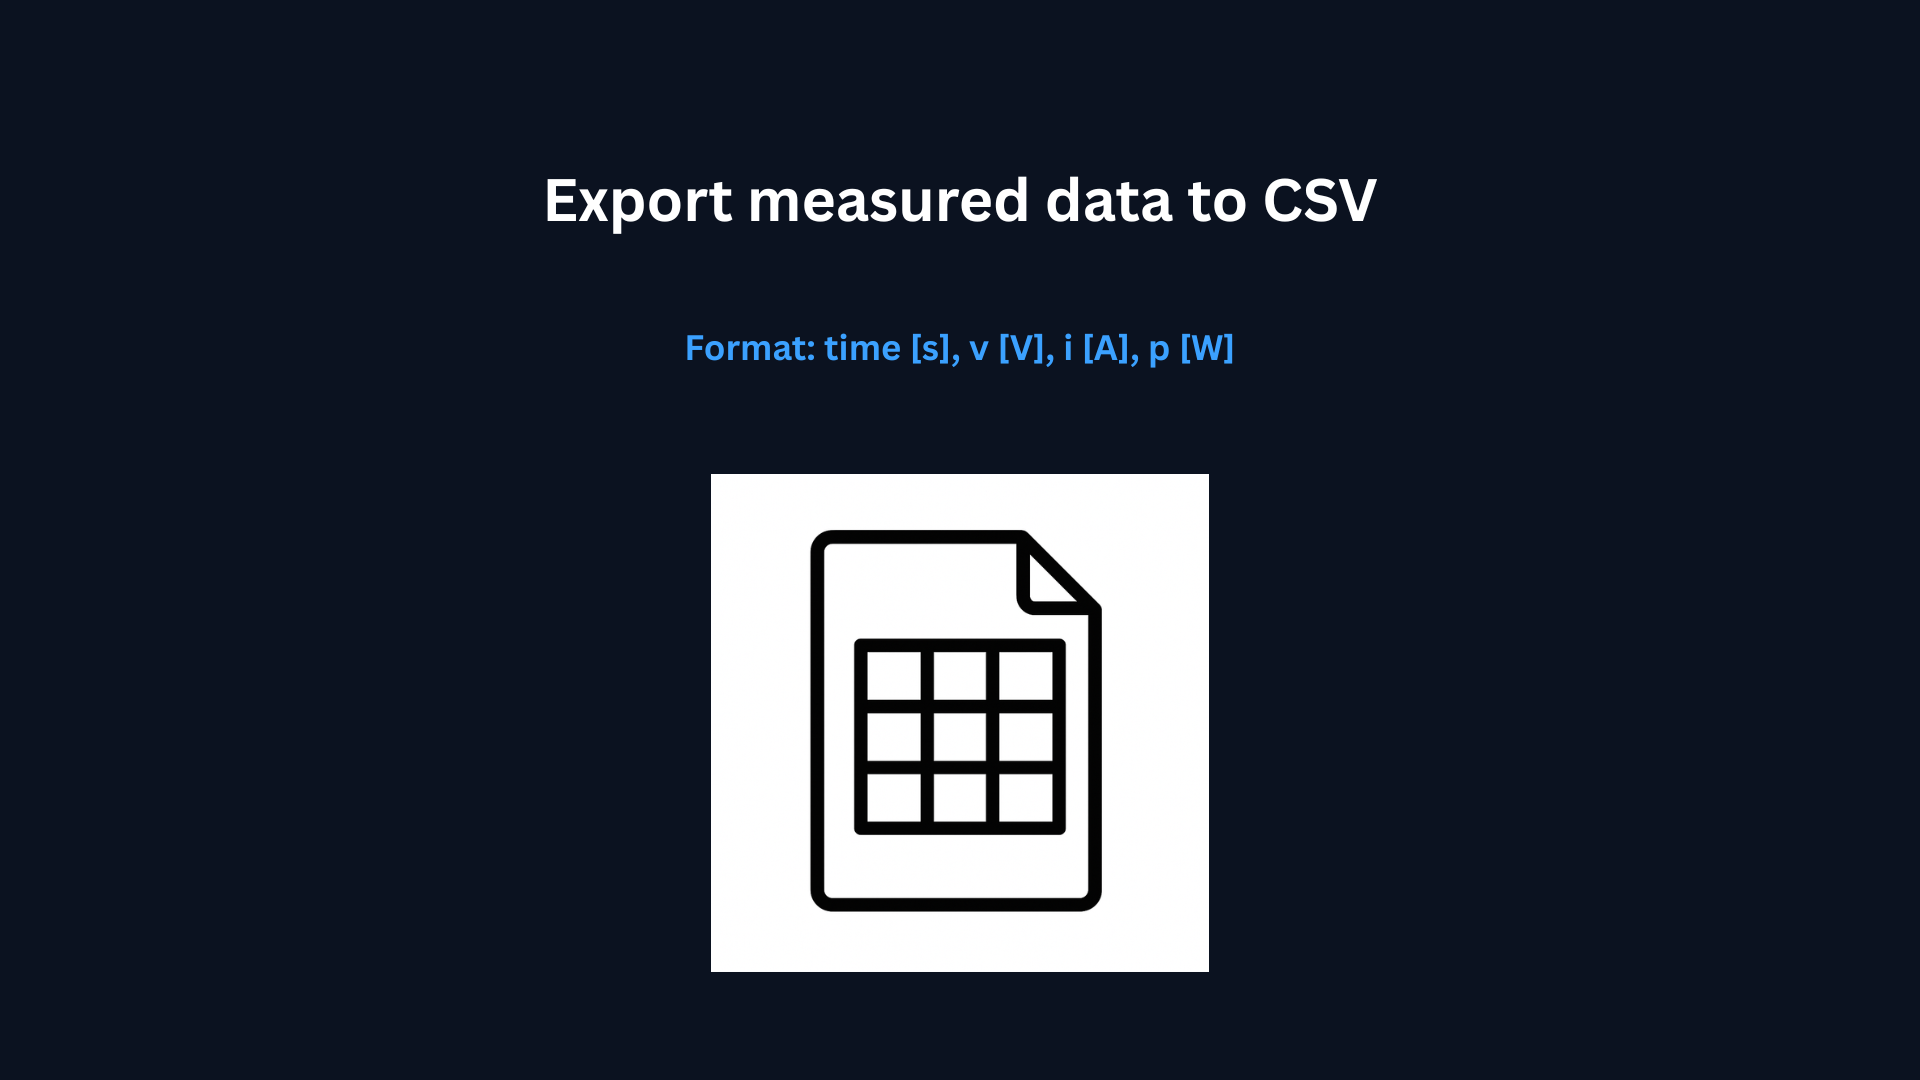
\includegraphics[width=0.22\textwidth]{6.png} &
        
\includegraphics[width=0.22\textwidth]{7.png} &
        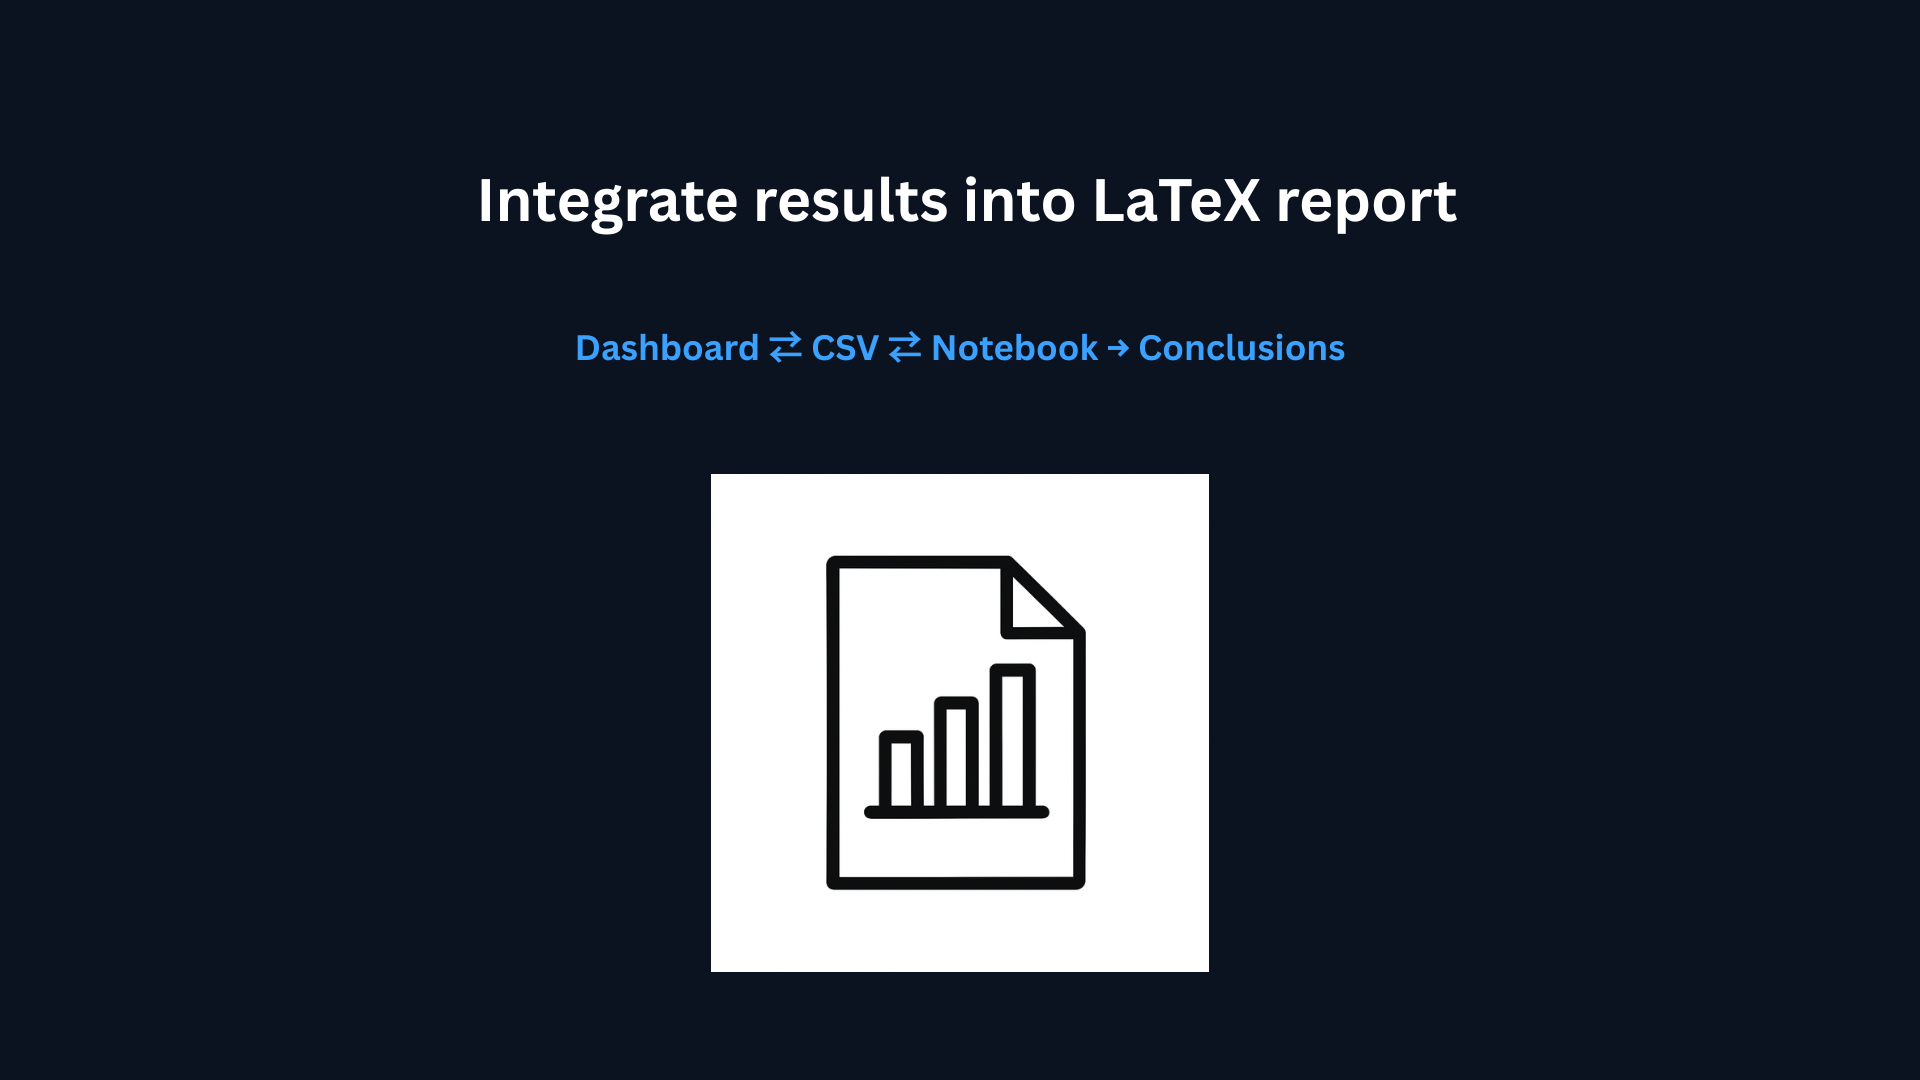
\includegraphics[width=0.22\textwidth]{8.png} \\
    \end{tabular}
    \caption{Storyboard of the animated infographic explaining the measurement
    process.}
    \label{fig:infographic_grid}
\end{figure}


\vspace{1cm}


\appendix
\section*{Appendix: AI Interactions}

Throughout the preparation of this report, AI tools (ChatGPT) were used in the
following ways:

\begin{itemize}
    \item \textbf{Exercise 1:} Assistance with LaTeX formatting, derivation
    layout, and clarifying the step-by-step application of Faraday’s law.
    \item \textbf{Exercise 2:} Guidance on LaTeX formatting for equations,
    checking the correctness of current and power expressions, and producing
    clean diagrams of AC elements.
    \item \textbf{Exercise 3:} Help with the structure of the measurement
    protocol, integration of figures into the report, and generating the LaTeX
    code to include multiple images in a storyboard. AI was also used to
    suggest clear wording for section introductions and conclusions.
    \item \textbf{General:} LaTeX formatting advice (headers, figures, tables),
    debugging minor errors, and ensuring consistent terminology.
\end{itemize}


\end{document}
